%% LyX 1.5.1 created this file.  For more info, see http://www.lyx.org/.
%% Do not edit unless you really know what you are doing.
\documentclass[english]{book}
\usepackage[T1]{fontenc}
\usepackage[latin9]{inputenc}
\pagestyle{headings}
\setcounter{secnumdepth}{3}
\setcounter{tocdepth}{3}
\usepackage{float}
\usepackage{textcomp}
\usepackage{graphicx}
\IfFileExists{url.sty}{\usepackage{url}}
                      {\newcommand{\url}{\texttt}}

\makeatletter

%%%%%%%%%%%%%%%%%%%%%%%%%%%%%% LyX specific LaTeX commands.
%% Bold symbol macro for standard LaTeX users
\providecommand{\boldsymbol}[1]{\mbox{\boldmath $#1$}}

%% Because html converters don't know tabularnewline
\providecommand{\tabularnewline}{\\}

%%%%%%%%%%%%%%%%%%%%%%%%%%%%%% Textclass specific LaTeX commands.
\newenvironment{lyxcode}
{\begin{list}{}{
\setlength{\rightmargin}{\leftmargin}
\setlength{\listparindent}{0pt}% needed for AMS classes
\raggedright
\setlength{\itemsep}{0pt}
\setlength{\parsep}{0pt}
\normalfont\ttfamily}%
 \item[]}
{\end{list}}

%%%%%%%%%%%%%%%%%%%%%%%%%%%%%% User specified LaTeX commands.
%% LyX 1.5.1 created this file.  For more info, see http://www.lyx.org/.
%% Do not edit unless you really know what you are doing.






\usepackage{float}

\usepackage{textcomp}

\usepackage{color}


\IfFileExists{url.sty}{\usepackage{url}
}
                      {\newcommand{\url}{\texttt}}

\makeatletter

%%%%%%%%%%%%%%%%%%%%%%%%%%%%%% LyX specific LaTeX commands.
%% Bold symbol macro for standard LaTeX users


%% Because html converters don't know tabularnewline


%%%%%%%%%%%%%%%%%%%%%%%%%%%%%% Textclass specific LaTeX commands.


%%%%%%%%%%%%%%%%%%%%%%%%%%%%%% User specified LaTeX commands.
%% LyX 1.5.4 created this file.  For more info, see http://www.lyx.org/.
%% Do not edit unless you really know what you are doing.






\usepackage{float}


\usepackage{textcomp}


\usepackage{url}




\makeatletter

%%%%%%%%%%%%%%%%%%%%%%%%%%%%%% LyX specific LaTeX commands.
%% Bold symbol macro for standard LaTeX users


%% Because html converters don't know tabularnewline


%%%%%%%%%%%%%%%%%%%%%%%%%%%%%% Textclass specific LaTeX commands.


%%%%%%%%%%%%%%%%%%%%%%%%%%%%%% User specified LaTeX commands.
%% LyX 1.5.4 created this file.  For more info, see http://www.lyx.org/.
%% Do not edit unless you really know what you are doing.



\usepackage{geometry}



\geometry{verbose,letterpaper,tmargin=1in,bmargin=1in,lmargin=1in,rmargin=1in}



\usepackage{float}



\usepackage{textcomp}



\usepackage{url}





\makeatletter

%%%%%%%%%%%%%%%%%%%%%%%%%%%%%% LyX specific LaTeX commands.
%% Bold symbol macro for standard LaTeX users



%%%%%%%%%%%%%%%%%%%%%%%%%%%%%% Textclass specific LaTeX commands.


%%%%%%%%%%%%%%%%%%%%%%%%%%%%%% User specified LaTeX commands.
\usepackage{hyperref}




\let\myUrl\url
\renewcommand{\url}[1]{(\myUrl{#1})}


\makeatother


\makeatother


\makeatother



\usepackage{babel}
\makeatother

\begin{document}
\noindent \begin{center}
\thispagestyle{empty}%
\begin{figure}[H]
 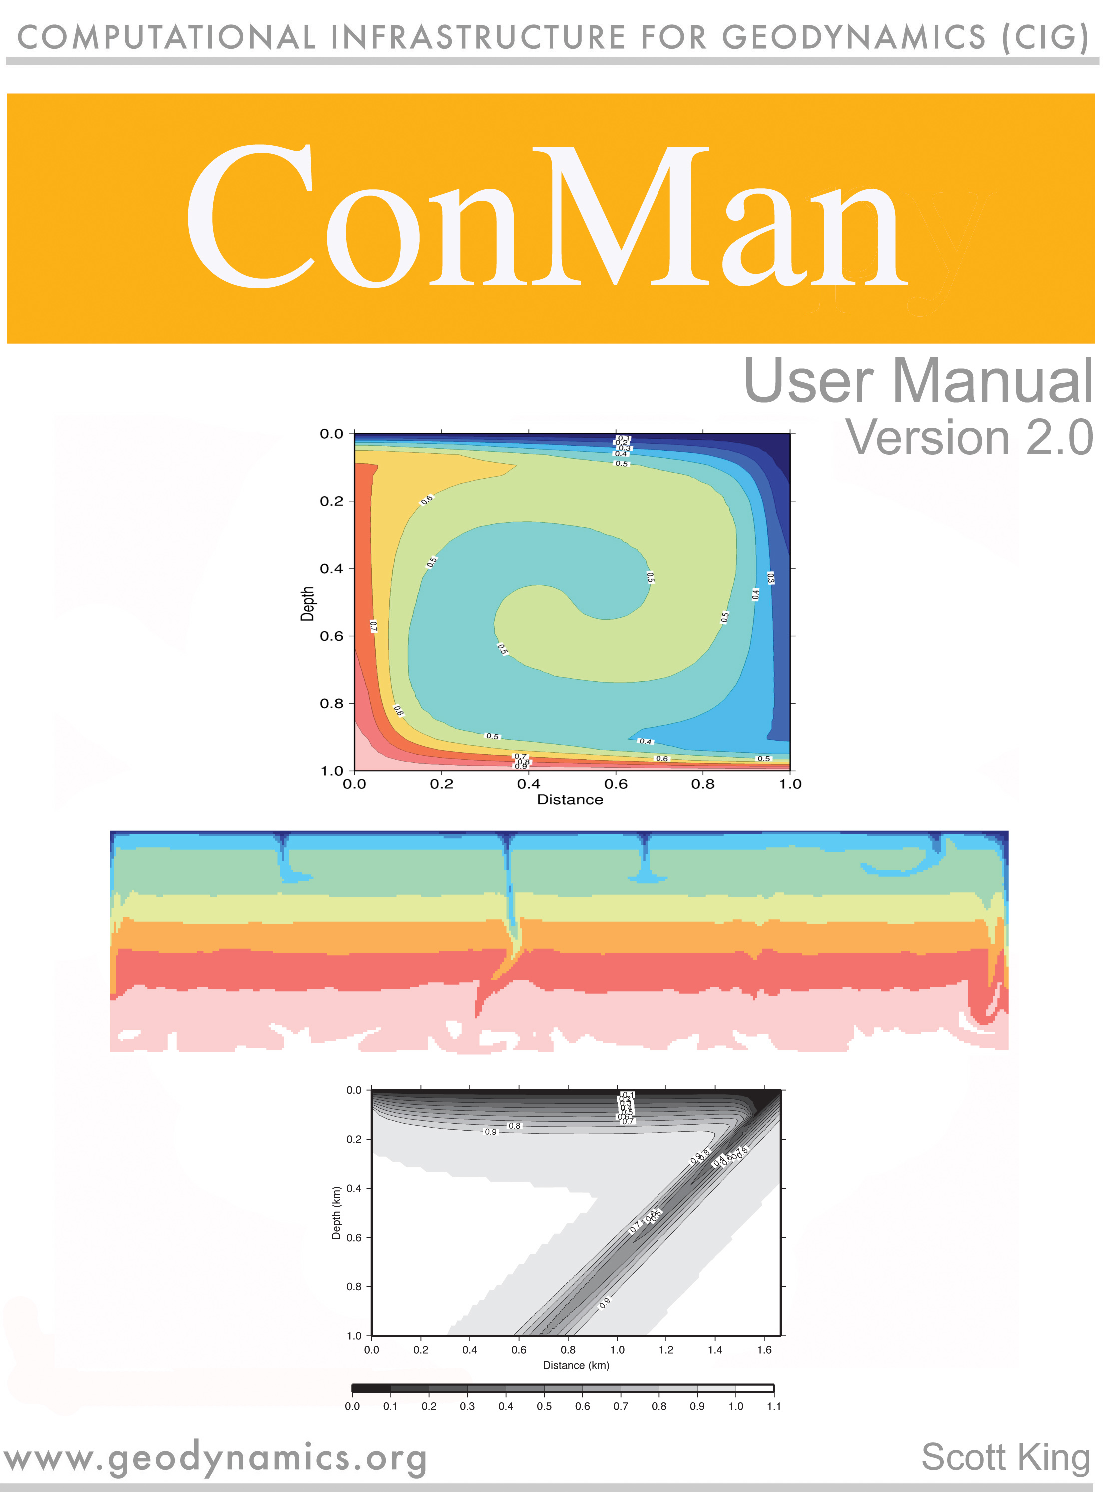
\includegraphics[width=0.75\paperwidth]{images/conman_cover} 
\end{figure}

\par\end{center}


\title{ConMan}


\author{� California Institute of Technology\\
 Scott King\\
 Version 2.0}


\date{\today}

\maketitle
\tableofcontents{}

\listoffigures


\raggedbottom

\newpage{}


\chapter{Preface}


\section{Abstract}

This manual serves as a user guide for ConMan, a vectorized finite
element program for the solution of the equations of incompressible,
infinite-Prandtl number convection in two dimensions originally written
by Arthur Raefsky, Scott King, and Brad Hager. ConMan is a public
domain program and is distributed free of charge to anyone who wishes
to use it and may be freely copied and modified. ConMan is written
in Standard Fortran 77 with cray pointers and runs on most Unix systems
with many Fortran compilers (see Section 3.4 \textbf{{[}TODO -- 3.4
is placeholder section. Is this correct? Need label to put cross ref
here]}). Porting it to other systems should be straightforward. As
with anything free it comes with no guarantees, but it has been benchmarked
against other existing codes (see Chapter \ref{cha:The-Benchmark-Cases}).
The authors would appreciate any information regarding bugs or potential
problems but make no promises regarding the timeliness of changes
or fixes; see Section \ref{sec:Support} for instructions on how to
report problems.


\section{Introduction}

This manual contains all of the necessary information for setting
up input and running ConMan. It assumes some familiarity with the
finite element method and Fortran. An excellent reference book for
more detail on the finite element method is \emph{The Finite Element
Method} by T.J.R. Hughes. All of the data structures and bookkeeping
arrays in ConMan follow the conventions in Hughes so for the person
who wishes to make extensive use of ConMan, this book is a worthwhile
investment.

This manual is broken up into several parts: it begins with a brief
introduction to the finite element method and the notation that is
used throughout the manual and ConMan. There is a discussion of the
equations solved and the material properties including how and where
to modify the code. There is also discussion of some key points concerning
the implementation and finally a description of all the input variables.
Within this document the following convention will be followed: subroutine
names from ConMan will be given in \textbf{bold} type, variables from
ConMan will be given in \emph{italicized} type.


\section{Citation}

Computational Infrastructure for Geodynamics (CIG) is making this
source code available to you in the hope that the software will enhance
your research in geophysics. The ConMan code was donated to CIG in
June 2008. A number of individuals have contributed a significant
portion of their careers toward the development of ConMan. It is essential
that you recognize these individuals in the normal scientific practice
by making appropriate acknowledgements.

The code is based on the method described in

\begin{itemize}
\item King, S.D., A. Raefsky, and B.H. Hager (1990), ConMan: Vectorizing
a finite element code for incompressible two-dimensional convection
in the Earth's mantle, \emph{Phys. Earth Planet. Int., 59,} 195-208. 
\end{itemize}
The code was originally developed by Scott King, Arthur Raefsky and
Brad Hager, although many people have contributed improvements to
ConMan over the past 15 years. The ConMan team requests that in your
oral presentations and in your papers that you indicate your use of
this code and acknowledge the author of the code and CIG \url{geodynamics.org}.


\section{Support}

ConMan maintenance is supported by a grant from the National Science
Foundation to CIG, managed by the California Institute of Technology,
under Grant No. EAR-0406751.

Any opinions, findings, and conclusions or recommendations expressed
in this material are those of the author and do not necessarily reflect
the views of the National Science Foundation.


\chapter{Computational Approach and Governing Equations}


\section{The Finite Element Method}

This section closely follows Hughes (\emph{The Finite Element Method})
Chapter~1, sections 1-4. There are two ways we can write the equation,
the strong and the weak form. More readers are probably more familiar
with the strong form, and less familiar with the weak form. The finite
element method is cast in the weak form. In elasticity, for example,
the weak form comes from a variational principal, such as the principal
of virtual displacements in elasticity. For viscous flow, there is
also a variational form, but we will not discuss that here.

In general, the finite element method takes a differential equation
(strong form) and transforms it into an integral equation (weak form).


\subsection{The Strong Form}

For example, the strong form of this simple equation is stated as
follows:

Given $f\left(x\right):\left[0,1\right]$ $\rightarrow\Re$ and constants
\emph{g} and \emph{h}, find $u:\left[0,1\right]\rightarrow\Re$, such
that

\begin{equation}
u,_{xx}\left(x\right)+f\left(x\right)=0\label{eq:}\end{equation}


\begin{equation}
u\left(1\right)=g\label{eq:}\end{equation}


\begin{equation}
-u,_{x}\left(0\right)=h\label{eq:}\end{equation}


\noindent This choice of initial conditions allows us to examine both
kinds of boundary conditions. The solution is trivial, but that does
not matter. For completeness, it is \begin{equation}
u(x)=g+(1-x)h+\int_{x}^{1}\left(\int_{0}^{y}f(z)dz\right)dy\end{equation}



\subsection{The Weak Form}

The weak form of the corresponding boundary value problem is stated:

Given \emph{f}, \emph{g} and \emph{h}, as before. Find $u\left(x\right)\epsilon\mathcal{L}$
such that for all $w\left(x\right)\epsilon\nu$

\begin{equation}
\intop_{0}^{1}w,_{x}\left(x\right)u,_{x}\left(x\right)=\intop_{0}^{1}w\left(x\right)f\left(x\right)dx+w\left(0\right)h\label{eq:}\end{equation}


\noindent $\nu$ is the set of weighting functions defined by

\begin{equation}
\nu=\left\{ w\left(x\right)|w\left(x\right)\epsilon H^{1},\, w\left(1\right)=0\right\} \label{eq:}\end{equation}


\noindent and $\mathcal{L}$ is a set of trial solutions defined by

\begin{equation}
\mathcal{L=\left\{ \mathrm{\mathit{u\left(x\right)|u\left(x\right)}\epsilon H^{1},\,\mathit{u}\left(1\right)=\mathit{g}}\right\} }\label{eq:}\end{equation}


\noindent $H^{1}$ is the set of all functions whose first derivatives
are square integrable on {[}0, 1]. The integral equation is then solved
by integrating over each element in the domain and adding the result.
The result is a large sparse matrix equation of the form

\begin{equation}
\left[K\right]x=b\label{eq:}\end{equation}


\noindent where \emph{{[}K]} is referred to as the element stiffness
matrix. There will be more to say about the implementation in Section
\ref{cha:Input-Guide}.


\subsection{Galerkin's Approximation}

Now we have a start on the finite element method. We continue to follow
Hughes; however, his notation becomes quite difficult to keep up with.
Now, let's begin to think about putting a solution on the computer.
Because we will have a finite approximation, related to how fine we
space our grid, our solution will only approximate the real solution.
Following Hughes' notation, the solution on the grid will be denoted
as $u^{h}$ where $h$ is some measure of the spacing at the grid.
Then, \begin{equation}
\int_{0}^{1}w^{h},_{x}u^{h},_{x}dx~=~\int_{0}^{1}w^{h}\, f^{h}\, dx+w^{h}(0)h.\label{eq:weak}\end{equation}
 approximates our exact solution $u$.

On a computer, we don't have a continuous solution. We have a solution
at discrete points. We need to approximate the solution between the
points (in order to integrate over the function). We will do this
with \textbf{shape functions}, as they are usually called in the finite
element language. Hughes uses $N_{A}A=1,2,\cdots,n$ to denote the
shape functions. You can also think of these as basis functions or
interpolation functions. We require $N_{A}(1)=0,A=1,2,\cdots,n$.
In order to specify our boundary condition, we need another shape
function which has the property \begin{equation}
N_{n+1}(1)=1.\end{equation}
 Then, $g^{h}$ is given by, \begin{equation}
g^{h}=gN_{n+1}\end{equation}
 and thus, \begin{equation}
g^{h}(1)=g.\end{equation}
 With these definitions, we can write our solution $u^{h}$ as \begin{equation}
u^{h}=\sum_{A=1}^{n}\, d_{A}\, N_{A}+gN_{n+1}\end{equation}
 where the $d_{A}$'s are unknown constants to be solved for.

In the next section we will make the shape functions more concrete.
It is useful to see how general this is, because in principle there
is a great deal of flexibility in how we choose the shape functions.

We have not said anything more about this function $w^{h}$ and how
we are going to choose it. If our shape functions form a basis set
for the grid, then we can represent \textbf{any} function as a sum
of the basis functions times some arbitrary coefficients $c_{i}$,
\begin{equation}
w^{h}=\sum_{A=1}^{n}\, c_{A}\, N_{A}=c_{1}\, N_{1}~+~c_{2}\, N_{2}~+~\cdots~+~c_{n}\, N_{n}\label{eq:whapprox}\end{equation}
 If you don't remember this part of your mathematics background think
of Fourier series. Any function one-dimensional function can be represented
as an infinite series of sines and cosines times some unique set of
coefficients. The shape functions form a similar kind of basis set.

Notice that because we required that $N_{A}(1)=0,A=1,2,\cdots,n$,
Equation~\ref{eq:whapprox} satisfies the requirement that $w^{h}(1)=0$,
as necessary.

Using our definitions of the $w^{h}$'s and our approximation for
$u^{h}$, we can get the messy expression for Equation~\ref{eq:weak}
\[
\int_{0}^{1}\left(\frac{\partial}{\partial x}\left(\sum_{A=1}^{n}\, c_{A}\, N_{A}\right)\frac{\partial}{\partial x}\left(\sum_{B=1}^{n}\, d_{B}\, N_{B}+gN_{n+1}\right)\right)dx~=~\]
 \begin{equation}
\int_{0}^{1}\sum_{A=1}^{n}\, c_{A}\, N_{A}\, f^{h}\, dx+\sum_{A=1}^{n}\, c_{A}N_{A}(0)h.\end{equation}
 By rearranging, we can write \begin{equation}
\sum_{A=1}^{n}G_{A}c_{A}=0\end{equation}
 where \[
G_{A}~=~\int_{0}^{1}\left(\frac{\partial N_{A}}{\partial x}\right)\left(\sum_{B=1}^{n}\, d_{B}\,\frac{\partial N_{B}}{\partial x}\right)dx\]
 \begin{equation}
-\int_{0}^{1}N_{A}\, f^{h}\, dx-N_{A}(0)h+\int_{0}^{1}\frac{\partial N_{A}}{\partial x}\frac{\partial N_{n+1}}{\partial x}\, g\, dx\end{equation}
 Now I use the fact that the shape functions are basis functions,
so $N_{A}\times N_{B}$ is zero except when $A=B$. We could equally
well use the fact that the $c_{A}$'s are arbitrary. Both of these
force us to conclude that each $G_{A}$ must be identically zero and
we get \[
\sum_{B=1}^{n}\,\left(\int_{0}^{1}\frac{\partial N_{A}}{\partial x}\frac{\partial N_{B}}{\partial x}\, dx\right)\, d_{B}=\]
 \begin{equation}
\int_{0}^{1}N_{A}\, f^{h}\, dx+N_{A}(0)h-g\,\int_{0}^{1}\frac{\partial N_{A}}{\partial x}\frac{\partial N_{n+1}}{\partial x}\, dx\label{eq:feform}\end{equation}
 Everything in Equation~\ref{eq:feform} is known except the $d_{B}$'s.
This constitutes a system of $n$ equations and $n$ unknowns. We
can think of the left-hand side as a matrix, $K_{AB}$ whose entries
are \begin{equation}
\int_{0}^{1}\frac{\partial N_{A}}{\partial x}\frac{\partial N_{B}}{\partial x}\, dx\label{eq:Kelements}\end{equation}
 We can write \begin{equation}
\sum_{B=1}^{n}\, K_{AB}d_{B}=F_{A},~~~~~A=1,2,\cdots,n\end{equation}
 or as a matrix equation \begin{equation}
\left[K\right]\,\{d\}=\{f\}\end{equation}
 where \begin{equation}
[k]=\left[\begin{array}{cccc}
K_{11} & K_{12} & \cdots & K_{1n}\\
K_{21} & K_{22} & \cdots & K_{2n}\\
\vdots & \vdots &  & \vdots\\
K_{n1} & K_{n2} & \cdots & K_{nn}\end{array}\right]\label{Kmatrix}\end{equation}
 By tradition, $\left[K\right]$ is the stiffness matrix, $\{f\}$
is the force vector, and $\{d\}$ is the displacement vector. When
the problem under consideration pertains to a mechanical system, this
makes the most sense, but even in heat conduction problems, or fluid
flow problems, the terminology is still (often) retained.


\subsection{Shape Functions}

At this point, we narrow the focus to deal with specifically the elements
in ConMan. It is possible to think very general shape functions, but
in practice, people use triangles or quadralaterals (in 2D). In terms
of the level of approximation, there are also a lot of possibilities.
We will stick to the simplest form, bilinear elements, but you should
be aware that higher order elements (biquadratic or bicubic spline
elements) are also popular with some people. This section is condensing
a lot of very useful material from Chapter 3 of Hughes' book into
a short overview. If you want to see more complete derivations, proofs
of convergence, etc., of how to go about using higher order elements,
look at Hughes book, Chapter 3.

Let's start by thinking of a rectangle that is 2a by 2b in length
centered at (0,0). There are two properties we would like the shape
functions to have \begin{eqnarray}
\sum_{A=1}^{4}N_{A}(X,Y) & = & 1\label{eq:normalize}\\
\sum_{A=1}^{4}N_{A}(X,Y)\, X_{A} & = & X\label{eq:interpx}\\
\sum_{A=1}^{4}N_{A}(X,Y)\, Y_{A} & = & Y\label{eq:interpy}\end{eqnarray}
 Equation~\ref{eq:normalize} says that they are normalized, so that
they sum to one (everywhere on X,Y). Equations~\ref{eq:interpx}
and~\ref{eq:interpy} state that the shape functions are also interpolation
functions. Without doing a lot of derivation, I will claim that for
the rectangle described above, \begin{eqnarray}
N_{1} & = & \frac{(a-x)(b-y)}{4ab}\\
N_{2} & = & \frac{(a+x)(b-y)}{4ab}\\
N_{3} & = & \frac{(a+x)(b+y)}{4ab}\\
N_{4} & = & \frac{(a-x)(b+y)}{4ab}\end{eqnarray}
 these shape functions satisfy the conditions in Equation~\ref{eq:normalize}
and Equations ~\ref{eq:interpx} and~\ref{eq:interpy}. A good exercise
would be to show this is true. A visual representation of these shape
functions is shown in Figure\ref{fig:The-bilinear-shape}.

\noindent \begin{center}
%
\begin{figure}
\caption{\label{fig:The-bilinear-shape}The bilinear shape function for a single
element (top) and the four elements whose shape functions combine
to form the global shape function for node A (bottom). Figure taken
from Hughes, Section 3.2.}


\noindent \begin{centering}
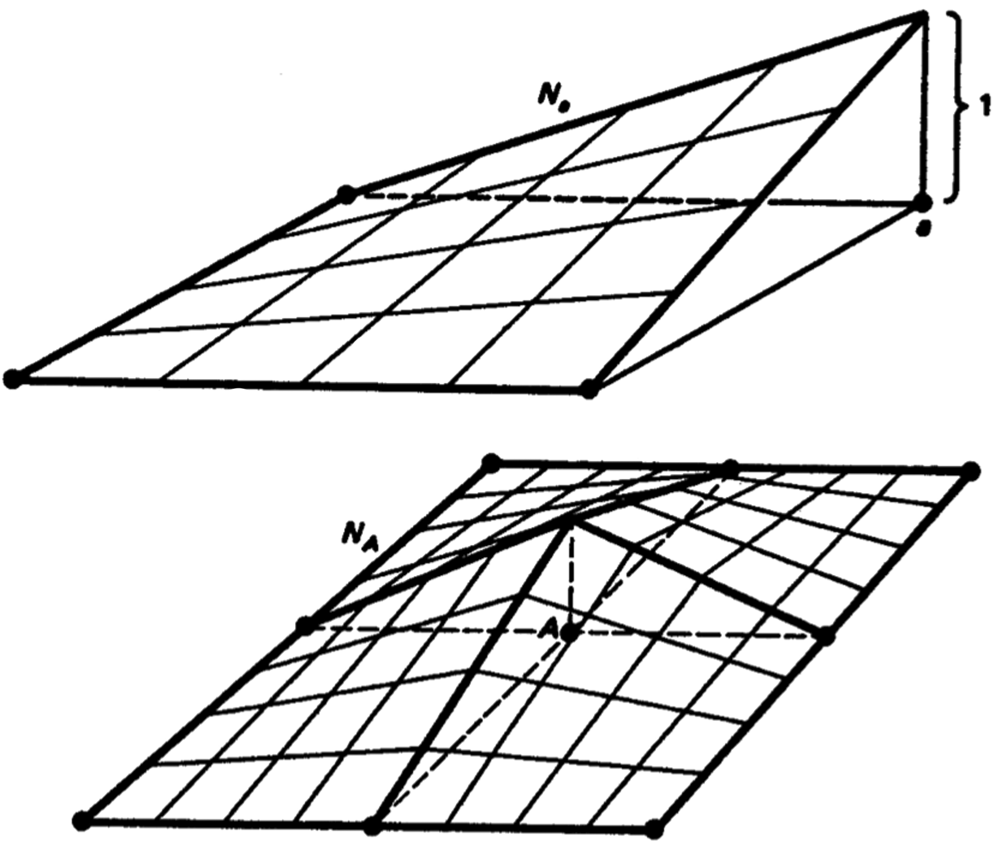
\includegraphics[scale=0.4]{images/conman-fig2} 
\par\end{centering}
\end{figure}

\par\end{center}

In ConMan we further choose to normalize this by setting $a=1$ and
$b=1$. This choice gives us an element whose area is 1, which is
a convenient way to think about things. (This is because we left the
factor of 1/4 in the denominator). In my code, to make one less set
of computations, I in effect set $a=0.5$ and $b=0.5$ so that the
denominator goes to 1.

Notice it is pretty easy to take derivatives of these shape functions
\begin{eqnarray}
N_{1,x} & = & \frac{-(1-y)}{4}\\
N_{2,x} & = & \frac{(1-y)}{4}\\
N_{3,x} & = & \frac{(1+y)}{4}\\
N_{4,x} & = & \frac{-(1+y)}{4}\end{eqnarray}
 \begin{eqnarray}
N_{1,y} & = & \frac{-(1-x)}{4}\\
N_{2,y} & = & \frac{-(1+x)}{4}\\
N_{3,y} & = & \frac{(1+x)}{4}\\
N_{4,y} & = & \frac{(1-x)}{4}\end{eqnarray}
 What do we do if we want to solve a problem on a domain that is not
convenient to split into a grid of 1 by 1 unit elements? We use an
important principle of mathematics, the Jacobian of the transformation
\begin{equation}
K_{11}~=~\int_{A}^{B}N_{1,x}N_{1,x}\, dx~=~\int_{0}^{1}N_{1,x}N_{1,x}\, Jdx\end{equation}
 where $J$ is the Jacobian of the transformation. This is a very
powerful point. When we are thinking of solving a regular Cartesian
domain, this just corresponds to a stretching or a shrinking (notice
we set $a=b=1$ above (see Figure \ref{fig:Figure-1}).

\noindent \begin{center}
%
\begin{figure}
\caption{\label{fig:Figure-1}The mapping between the global domain (right)
and the parent element domain (left) using the shape functions. Figure
taken from Hughes, Section 3.2.}


\noindent \begin{centering}
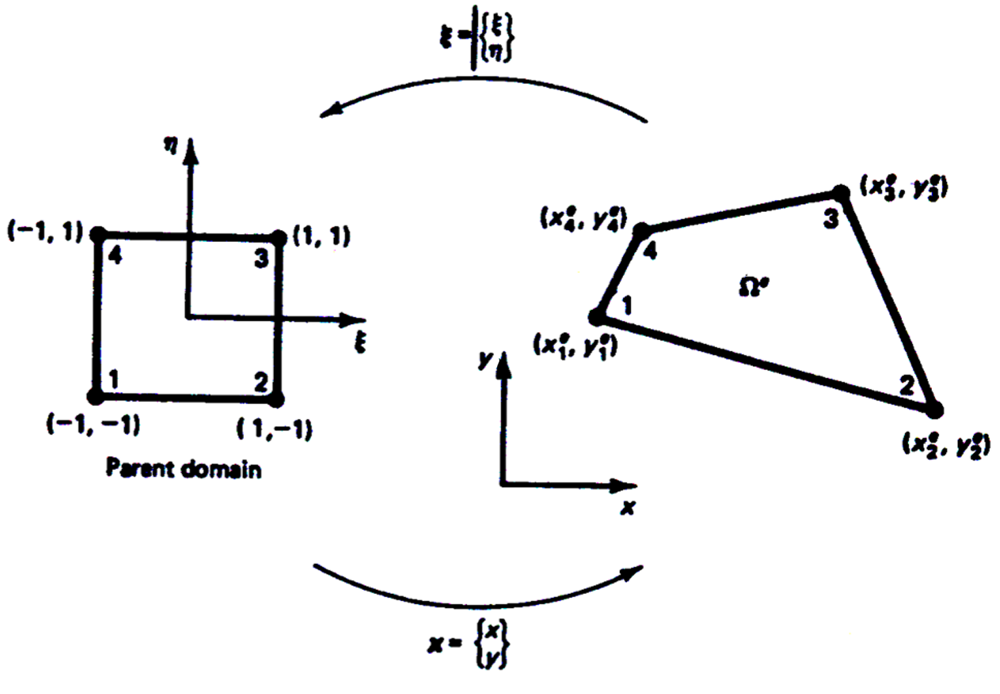
\includegraphics[scale=0.45]{images/conman-fig1} 
\par\end{centering}
\end{figure}

\par\end{center}

However, if we are thinking about a cylindrical geometry, for example,
we can use the Jacobian of the transformation between the geometries.
Let's look at two examples:

Converting an element 0.05 by 0.10 centered at (0.1,0.2) to the `parent
element' centered at (0,0). Hughes also uses $\xi,\eta$ for the $X,Y$
coordinate pair in the `parent element.' So we could write \begin{eqnarray}
x & = & 0.1+{0.05}\xi+0.0\eta\\
y & = & 0.2+{0.0}\xi+{0.10}\eta\end{eqnarray}
 or in matrix form we could write \begin{equation}
\left\{ \begin{array}{c}
x\\
y\end{array}\right\} =\left[\begin{array}{cc}
0.05 & 0.0\\
0.0 & 0.10\end{array}\right]\left\{ \begin{array}{c}
\xi\\
\eta\end{array}\right\} +\left\{ \begin{array}{c}
0.1\\
0.2\end{array}\right\} \label{eq:transform}\end{equation}
 If the transformation was from an arbitratry shaped quadrilateral
to the parent element, then the off diagonal terms in the matrix in
equation~\ref{eq:transform} will not be zero. It is easy enough
to show that \begin{equation}
\int_{x_{1}}^{x_{2}}\int_{y_{1}}^{y_{2}}f(x,y)\, dx\, dy=\int_{-1}^{1}\int_{-1}^{1}f(\xi,\eta)\,{\rm det}[J]\, d\xi\, d\eta\end{equation}
 where $[J]$ is the Jacobian of the transformation. It turns out,
and it is also easy to show, that ${\rm det}[J]$ is the ratio of
the areas when going from one rectangle to another (in fact any Cartesian
to Cartesian transformation).

\textbf{Advanced Topic:} Now suppose we want to map a cylindrical
domain to our `parent element.' We can use the same principle in this
case: \begin{eqnarray}
x & = & r\cos\theta=\cos\theta\,\xi-r\sin\theta\,\eta\\
y & = & r\sin\theta=\sin\theta\,\xi+r\cos\theta\,\eta\end{eqnarray}
 so \begin{equation}
{\rm det}[J_{geometry}]~=~r\cos^{2}\theta+r\sin^{2}\theta=r.\end{equation}
 of we would get \begin{equation}
\int_{r_{1}}^{r_{2}}\int_{\theta_{1}}^{\theta_{2}}f(r\cos\theta,r\sin\theta)\, r\, dr\, d\theta=\int_{-1}^{1}\int_{-1}^{1}f(\xi,\eta)\,{\rm det}[J_{area}]\, d\xi\, d\eta\end{equation}



\subsubsection{Gauss Quadrature}

An amazing fact, that makes the idea of finite elements easy and powerful,
is Gauss Quadrature. Gauss Quadrature is a way to turn an integral
into a summation. Let's begin with a 1D example, $f(x)=c$ \begin{equation}
\int_{-1}^{1}c\, dx=cx|_{-1}^{1}=2c\end{equation}
 Gauss noted that for any linear function \begin{equation}
\int_{-1}^{1}f(x)\, dx=2.0\times f(0)=2c\end{equation}
 For a linear function, $f(x)=ax+b$ \begin{equation}
\int_{-1}^{1}f(x)\, dx=f(\frac{-1}{\sqrt{3}})+f(\frac{-1}{\sqrt{3}})\end{equation}
 The direct way, \begin{equation}
\int_{-1}^{1}(ax+b)\, dx=(\frac{ax^{2}}{2}+bx)|_{-1}^{1}=\frac{a}{2}+b-(\frac{a}{2}-b)=2b\end{equation}
 Gauss' way \begin{equation}
\int_{-1}^{1}(ax+b)\, dx=a\frac{-1}{\sqrt{3}}+b+a\frac{1}{\sqrt{3}}+b=2b\end{equation}
 It turns out that $\frac{-1}{\sqrt{3}},\frac{1}{\sqrt{3}}$ are exact
for a linear equation, but from what I showed, so would any $-x,x$
combination, but what Gauss showed was more powerful, that if the
function is of higher order, the $\frac{-1}{\sqrt{3}},\frac{1}{\sqrt{3}}$
choice is the best approximation you can make with only two terms.
If we go to three terms, the choice would be $-\sqrt{\frac{3}{5}},0,\sqrt{\frac{3}{5}}$.

To integrate a 2D Cartesian region, like our parent element, it turns
out that 2 by 2 quadrature, or the four points \begin{eqnarray}
\xi=\frac{-1}{\sqrt{3}} & ~~~ & \eta=\frac{-1}{\sqrt{3}}\\
\xi=\frac{1}{\sqrt{3}} & ~~~ & \eta=\frac{-1}{\sqrt{3}}\\
\xi=\frac{1}{\sqrt{3}} & ~~~ & \eta=\frac{1}{\sqrt{3}}\\
\xi=\frac{-1}{\sqrt{3}} & ~~~ & \eta=\frac{1}{\sqrt{3}}\end{eqnarray}
 are sufficient to exactly integrate our bilinear shape functions
over the {-1,-1} to {1,1} domain.

At this point, it would be worth talking about the code ConMan for
a minute. The shape functions are generated in ConMan in the routine
\textbf{genshp} for GENerate SHape functions Parent domain. If you
look at the routine you will find the first part of it is pretty easy
to follow from the discussion above. Some of the second part is a
little tricky in the details, but generally it is also pretty easy
to follow.

The subroutine \textbf{genshg} deals with the global shape functions
(i.e., deals with the geometry and size). Originally, we called this
routine once and stored all the shape functions. As problem sizes
have grown, this took a lot of storage, so now we call it on the fly
for each element when needed. It is computationally more expensive
but cuts the storage requirement. This strategy will also be necessary
for a Lagrangian formulation or adaptive gridding.

There are two domains to keep in mind when thinking about the finite
element method: the global domain and the parent element domain (Figure
\ref{fig:Figure-1}). All calculations are done in the parent element
domain and the results are assembled into the global equations. This
means all calculations can be done for a single parent element. Elements
of different sizes or shapes filling an irregular global domain geometry
(i.e., non-rectangular) can be solved by the same program. The only
difference between these elements is the Jacobian of the transformation
between the input domain and the parent element domain, which is calculated
in routine \textbf{genshg}.

For ConMan the choice was made to use bilinear quadrilaterals as the
parent elements (Figure \ref{fig:The-bilinear-shape}). Higher order
elements (i.e., biquadratic or bicubic-spline) require more computational
work per element. It has been our experience that using grid refinement,
rather than using high-order elements, is the best strategy for an
efficient, accurate code for incompressible, advection-diffusion problems.

Because of the changing between domains, it is necessary to define
several bookkeeping arrays to identify nodes and elements in each
of the domains. It is worth noting that the numbering of local elements
always begins with 1 in the lower left-hand corner. There is no special
reason; you just have to choose a convention.

\begin{description}
\item [{{{{id}}}}] transforms global nodes to equation numbers (Figure
\ref{fig:Example-relationship-between}). 
\item [{{{{ien}}}}] transforms element local node numbers to global
node numbers (Figure \ref{fig:4-Example-relationship-between}). 
\item [{{{{lm}}}}] transforms element local node numbers to global
equation numbers. 
\end{description}
\noindent \begin{center}
%
\begin{figure}
\caption{\label{fig:Example-relationship-between} Example relationship between
global nodes and equation numbers for a 2 degree of freedom problem
using the id array. An equation number of zero denotes a boundary
condition. Figure taken from Hughes, Section 3.2.}


\noindent \begin{centering}
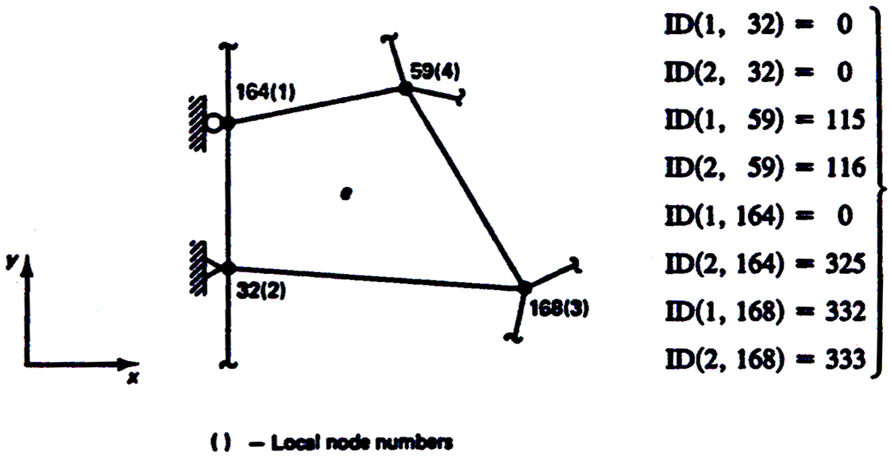
\includegraphics[scale=0.4]{images/conman-fig3} 
\par\end{centering}
\end{figure}

\par\end{center}

With these, the code is able to go back and forth between the parent
element domain and the global domain. Global node numbering is specified
by the user, and equation numbers are assigned by the code to denote
the row in the stiffness matrix corresponding to the degree(s) of
freedom for that node. One global node may have more than one equation
number (since there may be more than one degree of freedom per node).
Boundary conditions are specified with a zero equation number. Since
it is a sparse matrix, it is desirable to permute the stiffness matrix
for computational efficiency. These arrays spare the user from dealing
with the transformations, while making the code efficient.

\noindent \begin{center}
%
\begin{figure}
\caption{\label{fig:4-Example-relationship-between}Example relationship between
global node numbers and local element numbers using the ien array.
Local nodes are numbered counterclockwise from the bottom left-hand
corner. Figure taken from Hughes, Section 3.2.}


\noindent \begin{centering}
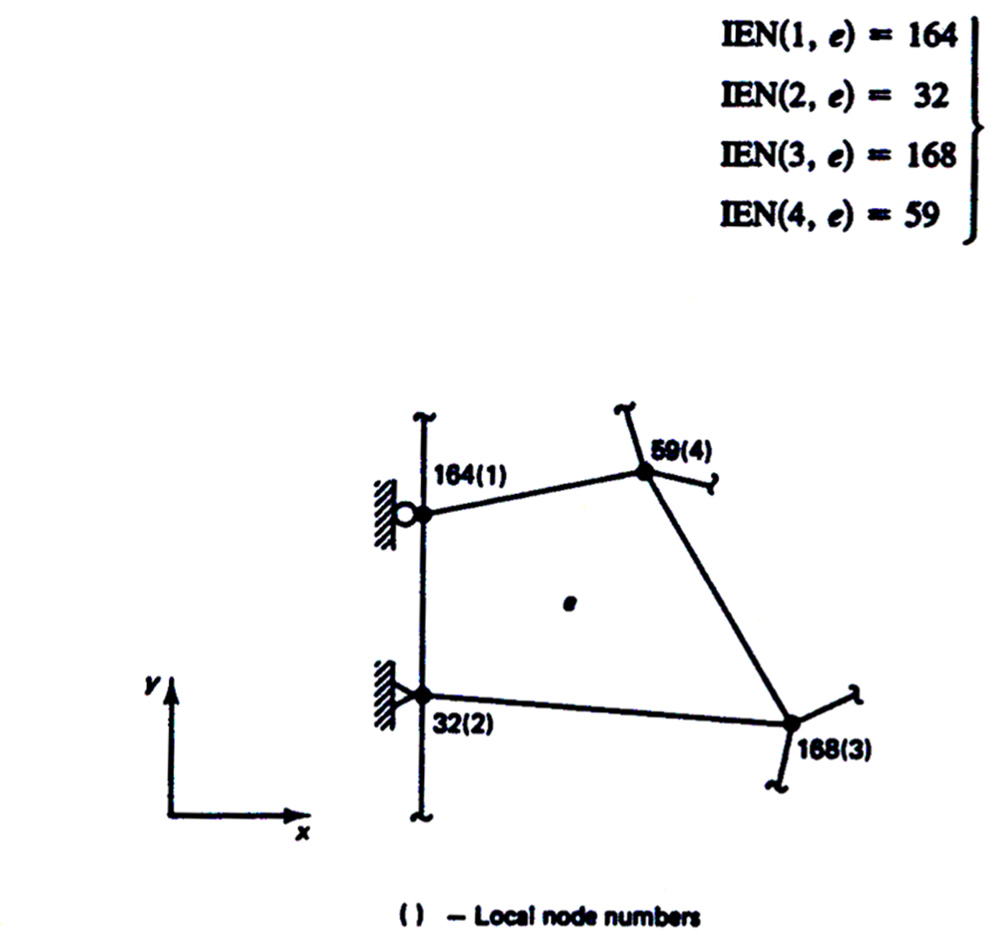
\includegraphics[scale=0.4]{images/conman-fig4} 
\par\end{centering}
\end{figure}

\par\end{center}

In the code, the data structures for these two arrays are

\begin{description}
\item [{{{{id}}}}] ( degree-of-freedom , global-node-number ) = equation-number 
\item [{{{{ien}}}}] ( local-node-number, element-number ) = global-node-number 
\item [{{{{lm}}}}] ( degree-of-freedom, local-node-number, element-number
) = global-equation-number 
\end{description}

\subsection{The Element Point of View}

Transforming between the element and global points of view is done
with the data structure called the IEN array for Element to Node transformation.
The IEN array takes an element number and a local node number, and
its value is the global node number. It is easiest to look at some
examples:

Consider a 3-element by 3-element grid. I will number my elements
and nodes starting in the lower left hand corner, and the node and
element numbers will increase linearly in the vertical direction.

\begin{verbatim} For element 3: ien (3, 1) = 3 ien (3, 2) = 7 ien
(3, 3) = 8 ien (3, 4) = 4

For element 5: ien (5, 1) = 6 ien (5, 2) = 10 ien (5, 3) = 11 ien
(5, 4) = 7 \end{verbatim}

There are three kinds of operations we might want to use. The first
is taking the values of some function (coordinates, velocities, temperatures,
stresses, etc.) defined on the global grid and getting the values
for a single element, which is called a {\em gather} operation.
The next is taking values in an element and spreading them out to
the global array, which is called a {\em scatter} operation. The
third operation is to take the value at a local node and add it to
the global value for that node, an {\em assembly} step.

All three operations -- gather, scatter, and assemble -- are done
by the routine \textbf{local}. Because it is called by the \textbf{genshp}
routine above, it is a good example to study.


\subsection{Equations}

\begin{eqnarray}
\tau_{ij,j}+f_{i} & = & 0\label{eq:motion}\\
u_{i,i} & = & 0\end{eqnarray}
 where \begin{equation}
\tau_{ij}=-p\delta_{ij}+2\mu u_{(i,j)}\label{eq:constit}\end{equation}
 where \begin{equation}
u_{(i,j)}=(u_{i,j}+u_{j,i})/2\end{equation}
 We replace Equation~\ref{eq:constit} with the following relationships
\begin{eqnarray}
\tau_{ij}=-p^{\lambda}\delta_{ij}+2\mu u_{(i,j)}\label{eq:constit-lam}\\
0=u_{i,i}+p^{\lambda}/\lambda.\label{eq:constit-lam2}\end{eqnarray}
 As $\lambda$ approaches infinity, these relations approach the incompressible
solution. Also, as $\lambda$ approaches infinity, $p^{\lambda}$
approaches the hydrostatic pressure in the incompressible case. In
general, the hydrostatic pressure is $-\tau_{ii}/3$. Substituting
Equation~\ref{eq:constit-lam2} into~\ref{eq:constit-lam} we get
\begin{equation}
\tau_{ij}=\lambda u_{i,i}\delta_{ij}+2\mu u_{(i,j)}\label{eq:constit-lam-final}\end{equation}
 or \begin{equation}
\tau_{ii}=3\lambda u_{i,i}+2\mu u_{i,i}\end{equation}
 or \begin{equation}
\tau_{ii}/3=-p=(\lambda+2/3\mu)u_{i,i}\end{equation}
 but we also have \begin{equation}
-p^{\lambda}=\lambda u_{i,i}\end{equation}
 from Equation~\ref{eq:constit-lam2}. Clearly in the incompressible
limit $\lambda\gg\mu$ then $\lambda+2/3\mu\rightarrow\lambda$ and
$p^{\lambda}\rightarrow p$. Also note that the continuity equation
is satisfied.

Now, substituting Equation~\ref{eq:constit-lam-final} into Equation~\ref{eq:motion}
we have \begin{equation}
\{\lambda u_{i,i}\delta_{ij}+2\mu u_{(i,j)}\},j+f_{i}=0\end{equation}
 At this point, it is probably easier to switch to differential notation.
These will also specialize to 2D: \begin{eqnarray}
\frac{\partial}{\partial x}\{\lambda(\frac{\partial u}{\partial x}+\frac{\partial v}{\partial z})+2\mu(\frac{\partial u}{\partial x}+\frac{\partial u}{\partial x})/2\}+\frac{\partial}{\partial z}\{2\mu(\frac{\partial v}{\partial x}+\frac{\partial u}{\partial z})/2\}+f_{x}=0\\
\frac{\partial}{\partial x}\{2\mu(\frac{\partial u}{\partial z}+\frac{\partial v}{\partial x})/2\}+\frac{\partial}{\partial z}\{\lambda(\frac{\partial u}{\partial x}+\frac{\partial v}{\partial z})+2\mu(\frac{\partial v}{\partial z}+\frac{\partial v}{\partial z})/2\}+f_{z}=0\end{eqnarray}


These are second order partial differential equations. Simplifying,
we get \begin{eqnarray}
\lambda(\frac{\partial^{2}u}{\partial x^{2}}+\frac{\partial^{2}v}{\partial x\partial z})+2\mu\frac{\partial^{2}u}{\partial x^{2}}+\mu(\frac{\partial^{2}u}{\partial z^{2}}+\frac{\partial^{2}v}{\partial z\partial x})+f_{x}=0\\
\lambda(\frac{\partial^{2}u}{\partial z\partial x}+\frac{\partial^{2}v}{\partial z^{2}})+\mu(\frac{\partial^{2}u}{\partial x\partial z}+\frac{\partial^{2}v}{\partial x^{2}})+2\mu\frac{\partial^{2}v}{\partial z^{2}}+f_{z}=0\end{eqnarray}


Now we use the same technique (approach) as we used in Possion's equation
to turn the differential form into an integral form. You can either
look at it as we find the variational form of the Stokes equation
(which is what we are doing) or you can think of it as multiplying
by a weighting function $w$ and integrating over the domain. Then
using integration by parts to convert the second derivatives to first
derivatives. This is done carefully by Hughes in \emph{The Finite
Element Method} on pages 197-200, but he has left out a number of
intermediate steps. Nothing about this step is hard, just tedious.
There is, however, a clever shortcut. If we return to the messy equations
at the top of the page, multiply them by the weighting function $w$
and integrate over the domain, then we do not have to use integration
by parts. To see this for yourself, simply take the equations directly
above this paragraph, multiply by a weighting function $w$ and integrate
over the 2D domain $\Omega$, then use integration by parts. You will
find (after a little algebra)

\begin{eqnarray}
\int\int_{\Omega}\frac{\partial w}{\partial x}\{\lambda(\frac{\partial u}{\partial x}+\frac{\partial v}{\partial z})+2\mu\frac{\partial u}{\partial x}\}+\frac{\partial w}{\partial z}\{2\mu(\frac{\partial v}{\partial x}+\frac{\partial u}{\partial z})/2\}\, d\Omega+\nonumber \\
\int\int_{\Omega}f_{x}\, w\, d\Omega=b.c.~terms\\
\int\int_{\Omega}\frac{\partial w}{\partial x}\{2\mu(\frac{\partial u}{\partial z}+\frac{\partial v}{\partial x})/2\}+\frac{\partial w}{\partial z}\{\lambda(\frac{\partial u}{\partial x}+\frac{\partial v}{\partial z})+2\mu\frac{\partial v}{\partial z}\}\, d\Omega+\nonumber \\
\int\int_{\Omega}f_{z}\, w\, d\Omega=b.c.~terms\end{eqnarray}
 Note that we don't get something for nothing; this shortcut does
not give us the boundary condition terms (velocity or flux). These
would fall out of the integration by parts. Recall, \begin{equation}
\int_{a}^{b}w\, dv=w\, v|_{a}^{b}-\int_{a}^{b}v\, dw\end{equation}
 where in our case $w$ is the weighting function and $v$ is the
second derivative term. The first term gives us the flux (first derivative)
boundary conditions. In the case of the momentum equations, that is
the applied tractions (or stress boundary conditions).

Now we make use of Galerkin's approximation, or more simply, we use
the same weighting functions as we use for interpolation function,
i.e., the shape functions, N. So we substitute \begin{eqnarray}
\frac{\partial w}{\partial x}=N_{x}\\
\frac{\partial w}{\partial z}=N_{z}\\
\frac{\partial u}{\partial x}=u\, N_{x}\\
\frac{\partial u}{\partial z}=u\, N_{z}\\
\frac{\partial v}{\partial x}=v\, N_{x}\\
\frac{\partial v}{\partial z}=v\, N_{z}\end{eqnarray}
 into our weak form equations. Although messy, that is straight-forward.
\begin{eqnarray}
\int\int_{\Omega}N_{x}\{\lambda(u\, N_{x}+v\, N_{z})+2\mu u\, N_{x}\}+N_{z}\{\mu(v\, N_{x}+u\, N_{z})\}\, d\Omega+\nonumber \\
\int\int_{\Omega}f_{x}\, w\, d\Omega=b.c.~terms\\
\int\int_{\Omega}N_{x}\{\mu(u\, N_{z}+v\, N_{x})\}+N_{z}\{\lambda(u\, N_{x}+v\, N_{z})+2\mu v\, N_{z}\}\, d\Omega+\nonumber \\
\int\int_{\Omega}f_{z}\, w\, d\Omega=b.c.~terms\end{eqnarray}


At this point, it is useful to separate the equations into a $\lambda$
part and a $\mu$ part. We can also write them as a 2D matrix equation
\begin{equation}
[K_{\lambda}]=\left[\begin{array}{cc}
N_{x}\lambda N_{x} & N_{x}\lambda N_{z}\\
N_{z}\lambda N_{x} & N_{z}\lambda N_{z}\end{array}\right]\label{eq:Klambda}\end{equation}
 and \begin{equation}
[K_{\mu}]=\left[\begin{array}{cc}
N_{x}2\mu N_{x}+N_{z}\mu N_{z} & N_{z}\mu N_{x}\\
N_{x}\mu N_{z} & N_{z}2\mu N_{z}+N_{x}\mu N_{x}\end{array}\right].\label{eq:Kmu}\end{equation}


Hughes makes use of an interesting and important observation. This
observation will greatly simplify constructing the stiffness matrix
for arbitrary coordinate systems. We can rewrite the stiffness matrices
above in the following form: \begin{equation}
[K_{\lambda}]+[K_{\mu}]=[B]^{T}[D][B]\label{eq:84}\end{equation}
 \begin{equation}
[D_{\lambda}]+[D_{\mu}]=[D]\end{equation}
 where \begin{equation}
[D_{\mu}]=\mu\left[\begin{array}{ccc}
2 & 0 & 0\\
0 & 2 & 0\\
0 & 0 & 1\end{array}\right]\end{equation}
 and \begin{equation}
[D_{\lambda}]=\lambda\left[\begin{array}{ccc}
1 & 1 & 0\\
1 & 1 & 0\\
0 & 0 & 0\end{array}\right]\end{equation}
 and \begin{equation}
[B]=\left[\begin{array}{cc}
N_{x} & 0\\
0 & N_{z}\\
N_{z} & N_{x}\end{array}\right].\end{equation}


The momentum and energy equations form a simple coupled system of
differential equations. We treat the incompressibility equation as
a constraint on the momentum equation and enforce incompressibility
in the solution of the momentum equation using a penalty formulation
described below. Since the temperatures provide the buoyancy (body
force) to drive the momentum equation and since there is no time-dependence
in the momentum equation, the algorithm to solve the system is a simple
one: Given an initial temperature field, calculate the resulting velocity
field. Use the velocities to advect the temperatures for the next
time step and solve for a new temperature field. If the time stepping
for the temperature equation is stable, then this method is stable
and converges as $\Delta t\rightarrow0$.

The element stiffness matrix (Equation~\ref{eq:84}) is made up of
the two terms from the left hand side of the integral equation. The
full element stiffness matrix for the quadralilateral element is an
8 by 8 matrix made up of 16 of the 2 by 2 matrices as shown in Figure~\ref{fig:8-The-storage-for}.
Because of symmetry we only need to form and store the upper triangular
part of the matrix. The integration is done using two by two gauss
quadrature, which is exact when the elements are rectangular and bilinear
shape functions are used. The $\lambda$ term is under-integrated
(one point rule) to keep the large penalty value from effectively
locking the element \cite{Malkus and Hughes 1978}. The right-hand
side is made up of three known parts, the body force term ($f_{i}$),
the applied tractions ($h_{i}$) and the applied velocities ($g_{i}$).
The momentum equation is equivalent to an incompressible elastic problem,
and the resulting stiffness matrix will always be positive definite
\cite[p. 84-89]{Hughes 1987}. This allows us to consider only the
upper triangular part of the stiffness matrix and save both storage
and operations using Cholesky factorization. More details of the method
and a formal error analysis can be found in \cite{Hughes et al 1979}.

The stiffness matrix is formed in routine \textbf{f\_vstf} and the
right-hand side is formed in routine \textbf{f\_tres}.

%\noindent \begin{center}
%\begin{figure}
%\caption{\label{fig:5-The-element-stiffness}The element stiffness matrix for
%the 2D Cartesian stokes equation. The 8 by 8 matrix is make up of
%16 2 by 2 submatrices of the form shown below. The $\lambda$ and
%$\mu$ parts are shown separately for clarity.}
%\noindent \begin{centering}
%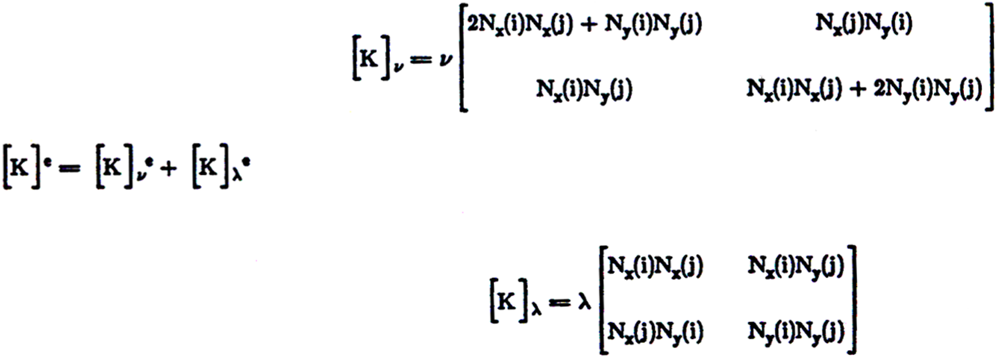
\includegraphics[scale=0.4]{images/conman-fig5.png} 
%\par\end{centering}
%\end{figure}
%\par\end{center}
%I'm not sure if we need this too...


\noindent \begin{center}
%
\begin{figure}
\caption{\label{fig:8-The-storage-for}The storage for the stiffness matrix
used in routine \textbf{f\_vstf}.}


\begin{centering}
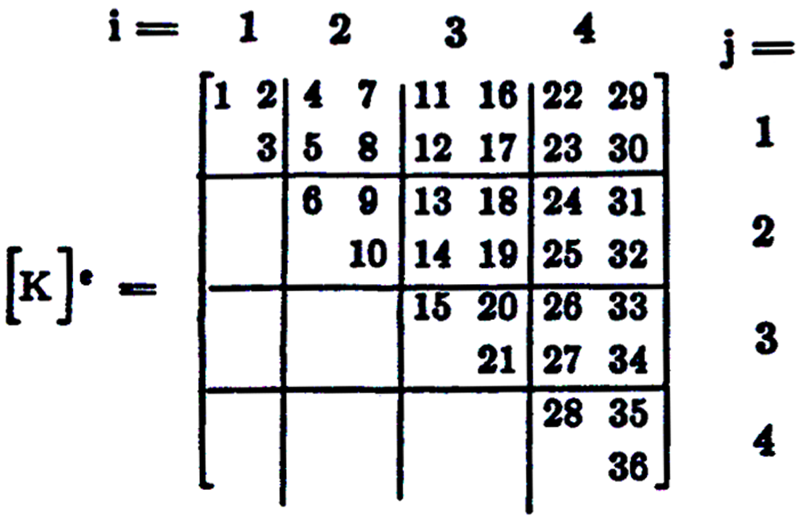
\includegraphics[scale=0.4]{images/conman-fig8} 
\par\end{centering}
\end{figure}

\par\end{center}

The energy equation is an advection-diffusion equation. The formal
statement is

Find $T:\Omega\rightarrow R$ such that

\begin{equation}
\dot{T}+u_{i}T_{,i}=\kappa T_{,ii}+H\,\,\,\,\,\, on\,\,\Omega\label{eq:}\end{equation}


\begin{equation}
T=b\,\,\,\,\,\, on\,\,\Gamma_{b}\label{eq:}\end{equation}


\begin{equation}
T_{,j}n_{j}=q\,\,\,\,\,\, on\,\,\Gamma_{q}\label{eq:}\end{equation}


\noindent where $T$ is the temperature, $u_{i}$ is the velocity,
$\kappa$ is the thermal diffusivity and $H$ is the internal heat
source. The weak form of the energy equation is given by

\begin{equation}
\int_{\Omega}\left(w+p\right)\dot{T}d\Omega=-\int_{\Omega}\left(w+p\right)\left(u_{i}T_{,i}\right)d\Omega\label{eq:}\end{equation}


\begin{equation}
-\kappa\int_{\Omega}w_{,i}T_{,i}d\Omega+\int_{\Gamma_{q}}wT_{,j}n_{j}d\Gamma_{q}\label{eq:}\end{equation}


\noindent where $\dot{T}$ is the time derivative of temperature,
$T_{,i}$ is the gradient of temperature, $w$ is the standard weighting
function and $\left(w+p\right)$ is the Petrov-Galerkin weighting
function with p, the discontinuous streamline upwind part of the Petrov-Galerkin
weighting function, given by

\begin{equation}
p=\tau u\nabla T=\tilde{k}\frac{u_{i}w_{,i}}{||u||^{2}}\label{eq:}\end{equation}


The energy equation is solved using Petrov-Galerkin weighting functions
on the internal heat source and advective terms to correct for the
under-diffusion and remove the oscillations which would result from
the standard Galerkin method for an advection dominated problem \cite{Hughes and Brooks 1979}.
The Petrov-Galerkin function can be thought of as a standard Galerkin
method in which we counterbalance the numerical underdiffusion by
adding an artificial diffusivity of the form

\begin{equation}
\left(\xi u_{\xi}h_{\xi}+\eta u_{\eta}h_{\eta}\right)/2\label{eq:}\end{equation}


\noindent with

\begin{equation}
\xi=1-\frac{2\kappa}{u_{\xi}h_{\xi}}\label{eq:}\end{equation}


\begin{equation}
\eta=1-\frac{2\kappa}{u_{\eta}h_{\eta}}\label{eq:}\end{equation}


\noindent where $h_{\xi}$ and $h_{\eta}$ are the element lengths
and $u_{\xi}$ and $u_{\eta}$ are the velocities in the local element
coordinate system ($\xi$ $\eta$ system) evaluated at the element
center. This form of discretization has no crosswind diffusion because
the {}``artificial diffusion'' acts only in the direction of the
flow (i.e., it follows the streamline), hence the name Streamline
Upwind Petrov-Galerkin (SUPG). This makes it a better approximation
than straight upwinding, and it has been demonstrated to be more accurate
than Galerkin or straight upwinding in advection dominated problems
\cite{Hughes and Brooks 1979}. It has recently been shown that the
SUPG method is one of a broader class of methods for advection-diffusion
equations referred to as Galerkin/Least-Squares methods \cite{Hughes et al 1988}.

The resulting matrix equation is not symmetric, but since the energy
equation only has one degree of freedom per node, while the momentum
equation has two or three, the storage for the energy equation is
small compared to the momentum equation. Since we use an explicit
time stepping method, the energy equation is not implemented in matrix
form. The added cost of calculating the Petrov-Galerkin weighting
functions is much less than the cost of using a refined grid with
the Galerkin method. The Galerkin method requires a finer grid then
the Petrov-Galerkin method to achieve stable solutions \cite{Travis et al 1990}.
Time stepping in the energy equation is done using an explicit predictor-corrector
algorithm. The form of the predictor-corrector algorithm is

Predict:

\begin{equation}
T_{n+1}^{\left(0\right)}=T_{n}+\Delta t\left(1-\alpha\right)\dot{T}_{n}\label{eq:}\end{equation}


\begin{equation}
\dot{T}_{n=1}^{\left(0\right)}=0\label{eq:}\end{equation}


Solve:

\begin{equation}
M^{*}\Delta\dot{T}_{n+1}^{\left(i\right)}=R_{n+1}^{\left(i\right)}\label{eq:}\end{equation}


\begin{equation}
R_{n+1}^{\left(i\right)}=-\left[\dot{T}_{n+1}^{\left(i\right)}+u\cdot\left(T_{n+1}^{\left(i\right)}\right),x\right]\left(w+p\right)-\label{eq:}\end{equation}


\begin{equation}
\tilde{k}w_{,x}\left(T_{n+1}^{\left(i\right)}\right),x+\,\,\,\left(boundary\, condition\, terms\right)\label{eq:}\end{equation}


Correct:

\begin{equation}
T_{n+1}^{\left(i+1\right)}=T_{n+1}^{\left(i\right)}+\Delta t\alpha\dot{T}_{n+1}^{\left(i\right)}\label{eq:}\end{equation}


\begin{equation}
\dot{T}_{n+1}^{\left(i+1\right)}=\dot{T}_{n+1}^{\left(i\right)}+\Delta\dot{T}_{n+1}^{\left(i\right)}\label{eq:}\end{equation}


\noindent where $i$ is the iteration number (for the corrector),
$n$ is the time-step number, $T$ is the temperature, $\dot{T}$
is the derivative of temperature with time, $\Delta\dot{T}$ is the
correction to the temperature derivative for the iteration, $M^{*}$
is the lumped mass matrix, $R_{n+1}^{\left(i\right)}$ is the residual
term, $\Delta t$ is the time step and $\alpha$ is a convergence
parameter. Note that in the explicit formulation $M^{*}$ is diagonal.

The time step is dynamically chosen, and corresponds to the Courant
time step (the largest step that can be taken explicitly and maintain
stability). With the appropriate choice of variables, $\alpha$ =
0.5 and two iterations, the method is second order accurate \cite[p. 562-566]{Hughes 1987}.

The predict step is done in routine \textbf{timdrv}, the residual
$R$ is formed in routine \textbf{f\_tres}, $M^{*}$ is formed in
routine \textbf{tmass}, and the correct step is also done in \textbf{f\_tres}.


\chapter{Implementation}


\section{Introduction}

There are generally two phases to ConMan, input and time stepping.
The main program is found in \textbf{ConMan.F}. The input is read
in the files \textbf{input.F and elminp.F}. Time stepping is doing
in \textbf{timdrv.F}. For legacy reasons, there is a rather complex
structure of \textbf{eglib} calling \textbf{eg2.F} which calls the
assembly and solve routines.

There are three significant differences that the user familiar with
past versions of ConMan will find in this version. The original version
of ConMan, distributed by King and/or Hager, was designed to take
advantage of machines with vector registers, such as the Cray X-MP
or Y-MP. Hence thoughout the code, operations that would be performed
on an individual element on a scalar machine were grouped together
so that they could be performed on a group of elements.

In this version of ConMan, the reordering of elements into blocks
with independent degrees of freedom and the reorganization of routines
into loops over element groups with inner do-loops having lengths
equal to the length of vector registers has been removed. This means
that the structure of the routines that form the element stiffness
matrix (\textbf{f\_vstf.F}) and right-hand side, or residual, (\textbf{f\_vres.F})
for the Stokes equation, and the routines for the calculation of the
right-hand side of the energy eqation (\textbf{f\_tmres.F}) are now
loops over elements with short inner loops over local element nodes
and/or integration points. One could argue that because modern CPU
is relying on fast cache to keep the arithmatic units busy, the kind
of grouping we did to take advantage of vector registers is still
useful for modern processors. However, the element reordering made
algorithms such as particle tracking (not implemented in this version)
more challenging and was difficult for users new to the finite element
method to understand. Therefore, we have removed the element reordering
and block vectorization.

The second major change is that we have implemented a Picard iteration
algorithm for steady-state problems (c.f. van Keken - thesis \textbf{{[}TODO:
This sounds different from the van Keken bib entry we have now. What
thesis?]}). Currently, this is implemented by changing compiler flags
in the Makefile. Picard iteration is an implicit solution to the energy
equation (as opposed to the predictor-corrector method described above);
hence, non-symmetric factor and back-solve routines have been added
as well as a routine to calculate the energy equation matrix and right-hand
side vectors (\textbf{f\_trhsimp.F}). To use Picard iteration you
change the variable $\alpha$ in the Time Sequence card (second line
of the input file) from 0.5 to 1.0 and change the iterations from
2 to 1 (same line). You need to {}``make clean'' and remake with
the target Picard, to generate a new executable (conman.pic). A future
revision may merge these energy equation solvers into a single code
and hide the need to change the iteration steps from the user. When
you have a steady-state solution, Picard iteration usually converges
in 10-100 steps, as opposed to several thousand steps. When there
is no steady-state solution, the Picard results are not useful and
the explicit solver should be used.

The third significant change is the replacement of the \textbf{mpoint}
function which allocated memory in the blank common array `a' with
the call \textbf{mmgetblk}. The `mm' routines are a fancy wrapper
around a c {\em malloc} call. The reason for this change is fairly
technical, and I will spare the user the details. The memory manager
source can be found in the directory \texttt{mm.src}. Care has to
be taken when compiling on 32-bit or 64-bit machines (change the header
file in \texttt{mm.src} from \texttt{mm2000\_32.h} to \texttt{mm2000\_64.h})
and change the compile flags in the Makefile. It is now possible to
use Fortran90's allocate routine for dynamic memory allocation, and
the memory manager should be removed in a future revision. Making
changes in the memory manager is tricky and this package is fragile.
Users who have a problem with the memory manager should request assistance
by contacting the CIG Mantle Convection Mailing List \url{cig-mc@geodynamics.org}.


\section{Material Properties}

As discussed above, the equations in dimensionless form have one dimensionless
parameter, the Rayleigh number.

\begin{equation}
Ra=\frac{g\alpha\Delta Td^{3}}{\kappa\mu}\label{eq:}\end{equation}


where $g$ is the acceleration due to gravity, $\alpha$ is the coefficient
of thermal expansion, $\Delta T$ is the temperature drop across the
box, $d$ is the depth of the box, $\kappa$ is the thermal diffusivity,
and $\mu$ is the dynamic viscosity. In ConMan, the input parameter
is the buoyancy part of the Rayleigh number.

\begin{equation}
Ra_{buoy}=g\alpha\label{eq:}\end{equation}


The depth, $d$, and the temperature difference, $\Delta T$ are specified
from the grid and the temperature boundary conditions. $\kappa$ and
$\mu$ are separate input parameters. If the depth, temperature difference,
$\kappa$ and $\mu$ are set to 1, then the buoyancy number, $RA_{buoy}$,
and the Rayleigh number, $Ra$, are the same.

The viscosity can be a function of temperature and/or depth. This
is done in routine \textbf{rheol}. The user can easily modify the
functional form for specific problems. The default functional form
is

\begin{equation}
\mu\left(T,Z\right)=\mu_{o}\left\{ \exp\left\{ \frac{E^{*}*1.0e3+V^{*}z}{R*(T+T_{o})}\right\} -\exp\left\{ \frac{E^{*}*1.0e3+V^{*}z}{R*(1+T_{o})}\right\} \right\} \label{eq:}\end{equation}


where $\mu_{o}$ is the preexponential viscosity, $E^{*}$ is the
activation energy, $V^{*}$ is the activation volume, $T_{o}$ is
the temperature offset, $T$ is the temperature and $z$ is the depth.
In the input files, $\mu_{o}$, is input on the viscosity card, $E^{*}$
is input as Tcon(1), $V^{*}$ is input as Tcon(2), and $T_{o}$ is
hardwired in \textbf{rheol.newt.F} to be 273. $\Delta T$ is hardwired
to be 2000.0.

The scaling in \textbf{rheol.newt.F} is such that $E^{*}$ can be
input in kJ/mole and $V^{*}$ can be input as cm$^{3}$.

Internal heating can be specified through the internal heating parameter.
If no bottom temperature is specified, the Rayleigh number becomes

\begin{equation}
Ra=\frac{g\alpha Hd^{5}}{k\kappa\mu}\label{eq:}\end{equation}


where $H$ is the internal heating parameter and $k$ is the thermal
conductivity. The grid can have multiple material groups, each with
its own set of material properties.


\section{Installation}

ConMan comes ready to run with a Unicos makefile. The file \textbf{Makefile}
contains the system calls for the compiler and the loader, FC and
LD respectively. These need to be changed for your machine. Also the
calls to \textbf{second}, a Cray timing routine, will have to be changed
in routine \textbf{timer}.


\section{Building from Source {[}TODO WEI -- thought you might need this section.
Or else delete]}


\subsection{System Requirements}

ConMan works on a variety of computational platforms and has been
tested on workstations running

\begin{itemize}
\item Mac OS X 10.4.6 (G4, G5, and Intel) 
\item Windows 2000 and XP SP2 
\item RedHat Fedora Core 5 (x86) 
\item OpenSuse 10.0 (x86) 
\item Gentoo (x86) 
\item Debian stable (x86 and AMD64), testing (x86), and unstable (x86) 
\end{itemize}
ConMan has also been tested on clusters running Redhat 7.2 (x86) and
RedHat Enterprise Linux 3 (EM64T).


\subsection{Dependencies}

This version of ConMan is self-contained and requires no external
libraries.


\subsection{\label{sec:Downloading-the-Code}Downloading the Code}

You can get the source for the latest release from the ConMan web
page \url{geodynamics.org/cig/software/packages/mc/conman/}. In that
tarball is the file ???name???.


\subsubsection{Source Code Repository (Experts Only)}

Advanced users and software developers may be interested in downloading
the latest ConMan source code directly from the CIG source code repository,
instead of using the prepared source package. To check whether you
have a subversion client installed on your machine, type:

\begin{lyxcode}
svn
\end{lyxcode}
You should get a response that looks something like this:

\begin{lyxcode}
Type~`svn~help'~for~usage.
\end{lyxcode}
Otherwise, you will need to download and install a Subversion client,
available at the Subversion Website \url{subversion.tigris.org/project_packages.html}.
Then the code can be checked out with the following command:

\begin{lyxcode}
svn~checkout~http://geodynamics.org/svn/cig/mc/3D/ConMan/trunk~ConMan
\end{lyxcode}

\section{\label{sec:Support}Support}

The primary point of support for ConMan is the CIG Mantle Convection
Mailing List \url{cig-mc@geodynamics.org}. Feel free to send questions,
comments, feature requests, and bugs to the list. The mailing list
is archived at

\begin{lyxcode}
cig-mc~Archives~\url{geodynamics.org/pipermail/cig-mc/}
\end{lyxcode}
You may also use the bug tracker

\begin{lyxcode}
Roundup~\url{geodynamics.org/roundup}
\end{lyxcode}
to submit bugs and requests for new features.


\chapter{\label{cha:Input-Guide}Input Guide}

To run ConMan a series of nine file names are needed, some for input
and some for output. Usually these are read from a runfile. The first
two files are input files \textbf{input} and \textbf{geom} and are
described in this section. The third file is an output file showing
all the input parameters in a verbose form. The fourth and fifth files
are an input temperature file (optional) and an output temperature
file. These are for starting a new run from a previous run. The sixth
file is a time series file (see routine \textbf{fluxke}), the seventh
file is the coordinates, velocities and temperatures, the eighth file
is for stresses (see routine \textbf{stress.F}) and the ninth file
is for geoid and topography (see routine \textbf{geoid.F}). These
file names are read in routine \textbf{ConMan.F}.

The input for ConMan is read from two different FORTRAN units. The
first unit, \textbf{iin}, contains the time stepping, output, and
material parameters as well as element type information while the
second unit, \textbf{igeom}, contains the coordinates, boundary values
and connectivity information. ConMan reads the file names to attach
to these units from standard input. The typical way to run ConMan
is to create a file with nine lines, one file name per line, and redirect
this into the executable (i.e., \% conman.pic < runfile \& ). \textbf{iin}
is attached to the file named on the first line and \textbf{igeom}
is attached to the file named on the second line (names must be ASCII
with a length less than 80 characters long).

The input deck was broken up so that an automatic grid generating
routine could be used to generate coordinates, boundary conditions
and element connectivities separate from ConMan. The only automatic
grid generation ConMan does is linear or bilinear interpolation which
is described in the appropriate sections of this guide.

The following sixteen cards or groups of cards are read from the \textbf{iin}
unit (throughout this guide a {}``card'' will mean one line of an
ASCII text file). These constitute the parameter part of the input
{}``deck'' for the program ConMan. The format for this guide is
a \textbf{bold} title line giving the card title followed by an \emph{italicized}
line showing the order of the parameters and a listing of the parameters
(with a brief explanation).

\begin{description}
\item [{{{{Title~Card}}}}] \emph{Any descriptive character string
up to 80 characters long} 
\item [{{{{Global~Constants~Card}}}}] \emph{numnp nsd ndof nelx
nelz mprec iflow necho inrsts iorstr nodebn ntimvs ntseq numeg isky
nwrap}

\begin{description}
\item [{{{{numnp}}}}] . . . . . . total number of nodal points 
\item [{{{{nsd}}}}] . . . . . . . . number of spatial dimensions
(always 2) 
\item [{{{{ndof}}}}] . . . . . . . number of degrees of freedom (always
2) 
\item [{{{{nelx}}}}] . . . . . . . number of elements in the x1 (horizontal)
direction 
\item [{{{{nelz}}}}] . . . . . . . number of elements in the x2 (vertical)
direction 
\item [{{{{mprec}}}}] . . . . . . precision flag (always use double)


1 - single

2 - double

\item [{{{{iflow}}}}] . . . . . . . data check flag


0 - check data only

1 - execute code

\item [{{{{necho}}}}] . . . . . . echo data flag


0 - minimum data echo (terse)

1 - echo data to output file (verbose)

\item [{{{{inrstr}}}}] . . . . . . . read restart file flag


0 - use default start (conductive)

1 - read restart file from unit 16

\item [{{{{iorstr}}}}] . . . . . . . write restart file flag


0 - don\textquoteright{}t write restart file

1 - write restart file to unit 17

\item [{{{{nodebn}}}}] . . . . . . number of edge nodes for nusselt
smoother 
\item [{{{{ntimvs}}}}] . . . . . . temperature dependent viscosity
flag


0 - stiffness matrix factored once

1 - stiffness matrix factored every time step

\item [{{{{ntseq}}}}] . . . . . . . number of time sequences (always
1)


currently only one supported

\item [{{{{numeg}}}}] . . . . . . number of element groups (always
1)


currently only one supported

\item [{{{{isky}}}}] . . . . . . . flag for skyline factor


0 - regular skyline

1 - vectorized skyline

\item [{{{{nwrap}}}}] . . . . . . number of nodes to wrap


equal to number of elements in vertical

to use nodes must be numbered increasing

fastest in vertical direction

\end{description}
\item [{{{{Time~Sequence~Cards}}}}] - ntseq cards


\emph{nstep niter alpha delt epstol}

\begin{description}
\item [{{{{nstep}}}}] . . . . . . . number of time steps 
\item [{{{{niter}}}}] . . . . . . . number of multicorrector iterations


2 - second-order expicit

1 - picard

\item [{{{{alpha}}}}] . . . . . . . multicorrector parameter


0.5 for explicit 2nd order

1.0 for picard

\item [{{{{delt}}}}] . . . . . . . time step (not used) 
\item [{{{{epstol}}}}] . . . . . . tolerance for hybrid method (not
used) 
\end{description}
\item [{{{{Output~Step~Card}}}}] \emph{nsdprt nsvprt nstprt nsmprt}

\begin{description}
\item [{{{{nsdprt}}}}] . . . . . . steps between disk output 
\item [{{{{nsvprt}}}}] . . . . . . steps between velocity output
(not used) 
\item [{{{{nstprt}}}}] . . . . . . steps between temperature, velocity
\& stress output 
\item [{{{{nsmprt}}}}] . . . . . . steps between stress field output
(not used) 
\end{description}
\item [{{{{Velocity~Boundary~Condition~Flag~Cards}}}}] \emph{bnode
enode incr (bcf(i), i=1,ndof)}

\begin{description}
\item [{{{{bnode}}}}] . . . . . . beginning node 
\item [{{{{enode}}}}] . . . . . . ending node 
\item [{{{{incr}}}}] . . . . . . . node increment 
\item [{{{{bcf(i)}}}}] . . . . . . . boundary condition flag for
ith degree of freedom


0 - free slip

1 - pinned degree of freedom

\end{description}
\end{description}
\emph{0 0 0 0 0 to end VBCF cards}

\begin{description}
\item [{{{{Temperature~Boundary~Condition~Flag~Cards}}}}] \emph{bnode
enode incr bcf}

\begin{description}
\item [{{{{bnode}}}}] . . . . . . beginning node 
\item [{{{{enode}}}}] . . . . . . ending node 
\item [{{{{incr}}}}] . . . . . . . node increment 
\item [{{{{bcf}}}}] . . . . . . . . boundary condition flag for temperature


1- fixed temperature

\end{description}
\emph{0 0 0 0 to end TBCF cards}

\item [{{{{Nusselt~Number~Boundary~Condition~Flag~Cards~-~Edge~Nodes}}}}] top
and bottom rows of nodes \emph{bnode enode incr}

\begin{description}
\item [{{{{bnode}}}}] . . . . . . beginning node 
\item [{{{{enode}}}}] . . . . . . ending node 
\item [{{{{incr}}}}] . . . . . . . node increment 
\end{description}
\emph{0 0 0 to end NNBCF (type a) cards}

\item [{{{{Nusselt~Number~Boundary~Condition~Flag~Cards~-~Second~Row~Nodes}}}}] second
from top and bottom rows of nodes \emph{bnode enode incr}

\begin{description}
\item [{{{{bnode}}}}] . . . . . . beginning node 
\item [{{{{enode}}}}] . . . . . . ending node 
\item [{{{{incr}}}}] . . . . . . . node increment 
\end{description}
\emph{0 0 0 to end NNBCF (type b) cards}

\item [{{{{Initial~Temperature~Card}}}}] \emph{pert xsize zsize}

\begin{description}
\item [{{{{pert}}}}] . . . . . . . perturbation from conductive state 
\item [{{{{xsize}}}}] . . . . . . . nondimensional length (x1 direction)
of box 
\item [{{{{zsize}}}}] . . . . . . . nondimensional height (x2 direction)
of box 
\end{description}
\item [{{{{Element~Parameter~Cards}}}}] - numeg cards \emph{ntype
numel nen nenl numat nedof numsuf nipt implv implt}

\begin{description}
\item [{{{{ntype}}}}] . . . . . . . element type


2 - two dimensional elements

\item [{{{{numel}}}}] . . . . . . total number of elements 
\item [{{{{nen}}}}] . . . . . . . . number of element nodes (always
4) 
\item [{{{{nenl}}}}] . . . . . . . number of local element nodes
(always 4) 
\item [{{{{numat}}}}] . . . . . . number of material groups 
\item [{{{{nedof}}}}] . . . . . . . number of element degrees of
freedom (always 2) 
\item [{{{{numsuf}}}}] . . . . . . number of imposed stress/flux
cards 
\item [{{{{nipt}}}}] . . . . . . . number of integration points per
element (always 5) 
\item [{{{{implv}}}}] . . . . . . . currently unused 
\item [{{{{implt}}}}] . . . . . . . currently unused 
\end{description}
\item [{{{{Viscosity~Card}}}}] \emph{visc(i), i=1,numat}

\begin{description}
\item [{{{{visc(i)}}}}] . . . . . . preexponential viscosity coefficient
for ith element 
\end{description}
\item [{{{{Penalty~Card}}}}] \emph{alam(i), i=1,numat}

\begin{description}
\item [{{{{alam(i)}}}}] . . . . . . penalty parameter for ith element 
\end{description}
\item [{{{{Diffusivity~Card}}}}] \emph{diff(i), i=1,numat}

\begin{description}
\item [{{{{diff(i)}}}}] . . . . . . . thermal diffusivity for ith
element 
\end{description}
\item [{{{{Buoyancy~Rayleigh~Number~Card}}}}] \emph{Ra(i), i=1,numat}

\begin{description}
\item [{{{{Ra(i)}}}}] . . . . . . . bouyancy part of Rayleigh number
for ith element 
\end{description}
\item [{{{{Internal~Heating~Parameter~Card}}}}] \emph{dmhu(i),
i=1,numat}

\begin{description}
\item [{{{{dmhu(i)}}}}] . . . . . . internal heat source for ith
material group 
\end{description}
\item [{{{{Activation~Energy~Card}}}}] \emph{tcon(1,i), i=1,numat}

\begin{description}
\item [{{{{tcon(1,i)}}}}] . . . . . activation energy for ith material
group for temperature dependent viscosity (kJ/mole) 
\end{description}
\item [{{{{Activation~Volume~Card}}}}] \emph{tcon(2,i), i=1,numat}

\begin{description}
\item [{{{{tcon(2,i)}}}}] . . . . . activation volume for ith material
group for temperature dependent viscosity (cm$^{3}$/mole) 
\end{description}
\item [{{{{Viscosity~Cutoff~Card}}}}] \emph{tcon(3,i), i=1,numat}

\begin{description}
\item [{{{{tcon(3,i)}}}}] . . . . . maximum value of the viscosity
for the ith material group 
\end{description}
\item [{{{{Surface~Force/Flux~Cards}}}}] - numsuf cards \emph{nel
side fnorm ftan flux}

\begin{description}
\item [{{{{nel}}}}] . . . . . . . . element number 
\item [{{{{side}}}}] . . . . . . . side to apply force and flux


1 - bottom

2 - right side

3 - top

4 - left side

\item [{{{{fnorm}}}}] . . . . . . . normal surface force 
\item [{{{{ftan}}}}] . . . . . . . tangential surface force 
\item [{{{{flux}}}}] . . . . . . . . heat flux 
\end{description}
\end{description}
The following four groups of cards are read from the \textbf{igeom}
unit. These constitute the geometry part of the input {}``deck''
for the program \texttt{conman}. The format of this section is the
same as above.


\section{Coordinate Group }

\begin{description}
\item [{{{{Absolute~Coordinate~Card}}}}] \emph{node gp (x(i,node)
i=1,nsd)}

\begin{description}
\item [{{{{node}}}}] . . . . . . . the node whose coordinates are
to be specified 
\item [{{{{gp}}}}] . . . . . . . . generation parameter for automatic
generation


0 - no autogeneration

2 - generate a line using node as a starting point

4 - generate a box using node as the lower left corner

\item [{{{{x(i,node)}}}}] . . . . . coordinate value in the ith spatial
dimension 
\end{description}
\item [{{{{Corner~Generation~Cards}}}}] - gp-1 cards \emph{node
mgen (x(i,node) i=1,nsd)}

\begin{description}
\item [{{{{node}}}}] . . . . . . . node number 
\item [{{{{mgen}}}}] . . . . . . . generation parameter


0 - don\textquoteright{}t use this as the start of a generation
sequence

1 - use this as the start of a generation sequence

\item [{{{{x(i,node)}}}}] . . . . . coordinate value in the ith spatial
dimension 
\end{description}
\item [{{{{Generation~Increment~Card}}}}] \emph{ninc1 inc1 ninc2
inc2}

\begin{description}
\item [{{{{ninc1}}}}] . . . . . . . number of additional nodes to
generate in x1 direction 
\item [{{{{inc1}}}}] . . . . . . . increment of nodes in x1 direction 
\item [{{{{ninc2}}}}] . . . . . . . number of additional nodes to
generate in x2 direction


0 - if gp equals 2

\item [{{{{inc2}}}}] . . . . . . . increment of nodes in x2 direction


0 - if gp equals 2

\end{description}
\emph{0 0 0 0 to end coordinate group}

\end{description}

\section{Velocity Boundary Condition Group }

\begin{description}
\item [{{{{Absolute~Velocity~Card}}}}] \emph{node gp (v(i,node)
i=1,nsd)}

\begin{description}
\item [{{{{node}}}}] . . . . . . . the node whose velocities are
to be specified 
\item [{{{{gp}}}}] . . . . . . . . generation parameter for automatic
generation


0 - no autogeneration

2 - generate a line using node as a starting point

4 - generate a box using node as the lower left corner

\item [{{{{v(i,node)}}}}] . . . . . velocity value in the ith spatial
dimension 
\end{description}
\item [{{{{Corner~Generation~Cards}}}}] - gp-1 cards \emph{node
mgen (v(i,node) i=1,nsd)}

\begin{description}
\item [{{{{node}}}}] . . . . . . . node number 
\item [{{{{mgen}}}}] . . . . . . . generation parameter


0 - don\textquoteright{}t use this as the start of a generation
sequence

1 - use this as the start of a generation sequence

\item [{{{{v(i,node)}}}}] . . . . . velocity value in the ith spatial
dimension 
\end{description}
\item [{{{{Generation~Increment~Card}}}}] \emph{ninc1 inc1 ninc2
inc2}

\begin{description}
\item [{{{{ninc1}}}}] . . . . . . . number of additional nodes to
generate in x1 direction 
\item [{{{{inc1}}}}] . . . . . . . increment of nodes in x1 direction 
\item [{{{{ninc2}}}}] . . . . . . . number of additional nodes to
generate in x2 direction

\begin{description}
\item [{{{{0}}}}] - if gp equals 2 
\end{description}
\item [{{{{inc2}}}}] . . . . . . . increment of nodes in x2 direction


0 - if gp equals 2

\end{description}
\emph{0 0 0 0 to end velocity group}

\end{description}

\section{Temperature Boundary Condition Group }

\begin{description}
\item [{{{{Absolute~Temperature~Card}}}}] \emph{node gp t(node)}

\begin{description}
\item [{{{{node}}}}] . . . . . . . the node whose velocities are
to be specified 
\item [{{{{gp}}}}] . . . . . . . . generation parameter for automatic
generation


0 - no autogeneration

2 - generate a line using node as a starting point

\item [{{{{t(node)}}}}] . . . . . . temperature value 
\end{description}
\item [{{{{Corner~Generation~Cards}}}}] - gp-1 cards \emph{node
mgen t(node)}

\begin{description}
\item [{{{{node}}}}] . . . . . . . node number 
\item [{{{{mgen}}}}] . . . . . . . generation parameter


0 - don\textquoteright{}t use this as the start of a generation
sequence

1 - use this as the start of a generation sequence

\item [{{{{t(node)}}}}] . . . . . . temperature value 
\end{description}
\item [{{{{Generation~Increment~Card}}}}] \emph{ninc1 inc1 ninc2
inc2}

\begin{description}
\item [{{{{ninc1}}}}] . . . . . . . number of additional nodes to
generate in x1 direction 
\item [{{{{inc1}}}}] . . . . . . . increment of nodes in x1 direction 
\item [{{{{ninc2}}}}] . . . . . . . number of additional nodes to
generate in x2 direction


0 - if gp equals 2

\item [{{{{inc2}}}}] . . . . . . . increment of nodes in x2 direction


0 - if gp equals 2

\end{description}
\emph{0 0 to end temperature group}

\end{description}

\section{Element Connectivity (ien) Generation Group }

\begin{description}
\item [{{{{Absolution~Element~Card}}}}] \emph{elnu ng mat no (ien(elnu,i)
i=1,nen)}

\begin{description}
\item [{{{{elnu}}}}] . . . . . . . element number 
\item [{{{{ng}}}}] . . . . . . . . generation parameter


0 - no generation

1 - generate using increments from increment card

\item [{{{{mat}}}}] no . . . . . . material number for this element 
\item [{{{{ien(elnu,i)}}}}] . . . . . global node number for the
ith local node of element counterclockwise from lower left corner 
\end{description}
\item [{{{{Increment~Card}}}}] \emph{nel1 incel1 incn1 nel2 incel2
incn2}

\begin{description}
\item [{{{{nel1}}}}] . . . . . . . number of elements in x1 (horizontal)
direction 
\item [{{{{incel1}}}}] . . . . . . . increment of elements in x1
(horizontal) direction 
\item [{{{{incn1}}}}] . . . . . . . increment of nodes in x1 (horizontal)
direction 
\item [{{{{nel2}}}}] . . . . . . . number of elements in x2 (vertical)
direction 
\item [{{{{incel2}}}}] . . . . . . . increment of elements in x2
(vertical) direction 
\item [{{{{incn2}}}}] . . . . . . . increment of nodes in x2 (vertical)
direction 
\end{description}
\emph{0 0 0 0 0 0 to end element connectivity group}

\end{description}

\chapter{\label{cha:Sample-Input-Files}Sample Input Files }

The lines below are a sample 50 element by 50 element input deck for
a 1 by 1 square, constant viscosity with the Picard method. This is
Blankenbach 1a:

\begin{lyxcode}
50~x~50~el.~plate~problem~from~Blankenbach~et~al.,~1989

~\#Nds~~sdm~dof~~~X~~~~Z~prc~ck~echo~rrst~wrst~nus~tdvf~tseq~nelg~sky~wr

~~2601~~2~~~2~50~~50~~~2~~1~~~~0~~~~0~~~~1~102~~~~0~~~~1~~~~1~~~1~~0

~time~step~information

~~~~100~~~1~~1.0~~1.0~~0.50000

~output~information

~~~~100~~~~100~~~~100~~~~100

~velocity~boundary~condition~flags:~IFCMT,DELNXTLN

~bnode~~~enode~~~incr~bcf1~bcf2

~~~~~1~~2551~~~~~51~~~~0~~~~1

~~2551~~2601~~~~~~1~~~~1~~~~0

~~~~~~1~~~51~~~~~~1~~~~1~~~~0

~~~~51~~2601~~~~~51~~~~0~~~~1

~~~~~1~~~~~1~~~~~~1~~~~1~~~~1

~~~~51~~~~51~~~~~~1~~~~1~~~~1

~~2551~~2551~~~~~~1~~~~1~~~~1

~~2601~~2601~~~~~~1~~~~1~~~~1

~~~~~~0~~~~~~0~~~~~~0~~~~0~~~~0

~temperature~boundary~condition~flags

~~~~~1~~2551~~~~51~~~~1

~~~~51~~2601~~~~51~~~~1

~~~~~~0~~~~~~0~~~~~~0~~~~0

~bndy~info~(top~-~bottom~rows)

~~~~~1~~2551~~~~51

~~~~51~~2601~~~~51

~~~~~~0~~~~~~0~~~~~~0

~bndy~info~(2nd~from~top~-~2nd~from~bottom~rows)

~~~~~~2~~2552~~~~51

~~~~~50~~2600~~~~51

~~~~~~0~~~~~~0~~~~~~0

~initial~condition~information

~~~~0.1~~~~1.0~~~~1.0~~~~1.0

~element~information

~2~~2500~4~4~1~2~0~5~0~0

~viscosity

~~1.0e0~~

~penalty~number

~~0.1E+08~

~diffusivity~(always~one)

~~~~1.0~~~

~Rayleigh~number

~~1.0e+04~~

~internal~heating~parameter

~~~~0.0

~~~~0.0

~~~~0.0~~~

~~~~1.0e7~~~
\end{lyxcode}
The lines below are a sample geometry file for the 50 by 50 element
problem.

\begin{lyxcode}
coordinates

~~~~~~1~~~~4~~0.0~~0.0

~~~2551~~~~1~~1.0~~0.0

~~~2601~~~~1~~1.0~~1.0

~~~~~51~~~~1~~0.0~~1.0

~~~~~50~~~51~~~50~~~~1

~~~~~~0~~~~0~~0.0~~0.0

~velocity~boundary~conditions~(non-zero)

~~~~~~0~~~~0~~0.0~~0.0

~temperature~boundary~conditions~(non-zero)

~~~~~~1~~~~2~~1.0

~~~2551~~~~0~~1.0

~~~~~50~~~51

~~~~~~0~~~~0~~0.0

~element~connectivity~and~material~groups

~~~~~~1~~~~~~1~~~~~~1~~~~~~1~~~~~52~~~~~53~~~~~~2

~~~~~50~~~~~50~~~~~51~~~~~50~~~~~~1~~~~~~1

~~~~~~0~~~~~~0~~~~~~0~~~~~~0~~~~~~0~~~~~~0~~~~~~0
\end{lyxcode}

\chapter{\label{cha:Output-Guide}Output Guide}


\section{The Output Files}

The output files names are taken from the names in the runfile. The
execution of \texttt{conman} proceeds by \% conman.pic < runfile where
the runfile has a list of filenames that can be up to 80 characters
long.

\noindent The names in the runfile are attached to the following input
or output files.

\begin{lyxcode}
input~

geometry~

output~

restart~input~

restart~output~

time~series~output~

temperature~(and~velocity)~

field~output~stress~(and~viscosity)~

field~output~geoid~output~
\end{lyxcode}
All files are ASCII files. The {\em input} and {\em geometry}
files are as described in the previous section.

The {\em output} file is a formatted record of the input. If the
variable {\em necho} is set to one, then values of the coordinates
and boundary conditions are output and the file can become large.
Near the end of the {\em output} file execution time is listed
for various subparts of the code.

The {\em restart input} file is an input file that is used if the
variable {\em inrstr} is set to one. The file is ASCII but formatted
and the format statement can be found in the file \textbf{input.F}.
The first line contains the initial timestep and time, the second
line is a header, and the third through {\em numnp} lines contains
the node, temperature and time derivative of temperature.

The {\em restart output} file is an output file that is used if
the variable {\em iorstr} is set to one. We recommend this always
be set to run. This file is overwritten every {\em nsdprt} steps
and the output is written from the file \textbf{timdrv.F}

The {\em time series output} file is written every time step. The
values are ASCII and are heat flux at the bottom, heat flux at the
top, kinetic energy, and time. All values are dimensionless. This
file is written from the routine \textbf{fluxke.F}

The {\em Temperature and velocity output} file is an ASCII file
written from the routine \textbf{print.F}. There are two header lines
that contain {\em nsd, nelx, nelz, numnp, nstep, time}. The second
line labels the output and the third through numnp lines list the
node, x, z, vx, vz, and temperature values at each node. This file
is output every {\em nsvprt} steps and each successive set of values
is appended to the end of the file. The unix command {\em split
-{numnp+2} tempfile} can be used to split the file into files that
are {\em numnp+2} lines long.

The {\em Stress output} file is an ASCII file written from the
routine \textbf{prtstr} which can be found in the file \textbf{stress.F}.
Like the temperature velocity file there are two header lines that
contain {\em nsd, nelx, nelz, numnp, nstep, time}. The second line
labels the output and the third through \texttt{numnp} lines list
the node, x, z, txx, tzz. txz. p and viscosity at each node. This
file is output every {\em nsvprt} steps and each successive set
of values is appended to the end of the file. The unix command {\em
split -{numnp+2} tempfile} can be used to split the file into files
that are {\em numnp+2} lines long.

The {\em geoid output} file contains the horizontal coordinate,
the dynamic topography, the geoid contribution from the temperature
only and the total geoid (from surface and cmb topography, and internal
(i.e., temperature) density contrasts). This is written from the file
\textbf{geoid.F}. The dimensional values are hard wired into the code
and can be found at the top of \textbf{geoid.F}. This version of the
geoid code has not been tested with flow-through boundary conditions
(i.e, {\em nwrap = nelz}).

{\em \textbf{\textcolor{red}{Warning.}} As written, the code assumes
a Rayleigh number of $10^{7}$ and does not adjust the parameters
as the Rayleigh number changes. This would be a trivial fix but still
may not yield the results intended. It is best to carefully check
the \textbf{geoid.F} source for the specific problem if interest.}


\chapter{\label{cha:The-Benchmark-Cases}The Benchmark Cases}

We provide input and geometry files for the benchmark cases described
below in the directories \texttt{cookbook1} and \texttt{cookbook2}.


\section{Cookbook 1: Constant Viscosity Benchmark for ConMan}

Here we reproduce the results from Blankenbach et al. (1989) \textbf{{[}TODO
need reference for bibliography]} for constant viscosity in a unit-aspect
ratio domain, with free-slip boundary conditions, heated from below
and cooled from above. The user should note that to run this problem,
you will need to modify the routines \textbf{rheol.newt.F} and \textbf{geoid.F}
following the comments in those routines. The constant viscosity calculations
(1a, 1b, and 1c) use a Rayleigh number of $10^{4}$, $10^{5}$, and
$10^{6}$ respectively and the dimensional parameters are listed in
Table~\ref{tab:Mantle-parameters-for}. The time is the runtime in
seconds for the Picard version of the code using 100 iterations on
an intel MacPro with two 3~GHz processors using the Intel fortran
compiler with -O2 optimization. While the problems in Blankenbach
et al. are specified dimensionally, the equations are solved non-dimensionally
within ConMan for numerical stability and the scaling factors are
applied to the results.

The results are computed on uniformly spaced grids and the global
properties of Nusselt number and root-mean-square velocity, as well
as the topography and geoid at the left- and right-hand side of the
domain are reported, along with the extrapolated value from Christensen's
results (see Blankenbach et al., 1989 for discussion) in Table~\ref{tab:Blankenbach-(1989)-Benchmark-1a}
(Rayleigh number $10^{4}$), Table~\ref{tab:Blankenbach-(1989)-Benchmark-1b}
(Rayleigh number $10^{5}$), and Table~\ref{tab:Blankenbach-(1989)-Benchmark-1c}
(Rayleigh number $10^{6}$). For the global properties of Nusselt
number and root-mean-square velocity, the 50 by 50 element grid are
within 1\% of Christensen's extrapolated results even for the Rayleigh
number $10^{6}$ calculations. The agreement for the point values
of topography and geoid are also 1\% error on the 50 by 50 grid for
the topography and geoid for the 50 by 50 element grid for the Rayleigh
number $10^{6}$ calculations (Table~7.4). For the 200 by 200 grid,
all values converge to Christensen's extrapolated results.

%
\begin{table}[htdp]
 

\begin{centering}
\begin{tabular}{lccc}
\hline 
\multicolumn{1}{c}{Parameter} & \multicolumn{1}{c}{Symbol} & \multicolumn{1}{c}{Value} & \tabularnewline
\hline 
depth of domain  & $d$  & $10^{6}$~m  & \tabularnewline
gravitational acceleration  & g  & 10 m/s$^{2}$  & \tabularnewline
temperature difference  & $\Delta T$  & 1000 K  & \tabularnewline
density  & $\rho$  & 4000~kg m$^{-3}$  & \tabularnewline
thermal diffusivity  & $\kappa$  & $1.0\times10^{-6}$ m$^{2}$ s$^{-1}$  & \tabularnewline
coefficient of thermal expansion  & $\alpha$  & $2.5\times10^{-5}$  & \tabularnewline
kinematic viscosity  & $\eta$  & $2.5\times10^{19}$ Pa s (1a)  & \tabularnewline
\null  & \null  & $2.5\times10^{18}$ Pa s (1b)  & \tabularnewline
\null  & \null  & $2.5\times10^{17}$ Pa s (1c)  & \tabularnewline
gravitational constant  & $G$  & $6.673\times10^{-11}$  & \tabularnewline
\hline
\end{tabular}
\par\end{centering}

\caption{\label{tab:Mantle-parameters-for}Mantle parameters for Blankenbach
constant viscosity benchmarks.}


\label{default} 
\end{table}


%
\begin{table}
\centering \begin{tabular}{|rccccccr|}
\hline 
\multicolumn{1}{|c}{Grid} & \multicolumn{1}{c}{V$_{rms}$} & \multicolumn{1}{c}{Nusselt No.} & \multicolumn{1}{c}{Topo$_{L}$} & \multicolumn{1}{c}{Topo$_{R}$} & \multicolumn{1}{c}{Geoid$_{L}$} & \multicolumn{1}{c}{Geoid$_{R}$} & \multicolumn{1}{c|}{Run Time (sec)}\tabularnewline
\hline 
50  & 42.906  & 4.887  & 2261.956  & -2911.473  & 55.346  & -63.178  & 1.98 \tabularnewline
100  & 42.875  & 4.885  & 2256.094  & -2905.356  & 54.957  & -62.765  & 18.04 \tabularnewline
200  & 42.867  & 4.885  & 2254.541  & -2903.763  & 54.856  & -62.658  & 187.43 \tabularnewline
\hline 
\dag C$_{ext}$  & 42.865  & 4.884  & 2254.021  & -2903.221  & 54.822  & -62.622  & \null \tabularnewline
\hline 
\multicolumn{8}{|l|}{\dag Christensen's extrapolated values.}\tabularnewline
\hline
\end{tabular}

\caption{\label{tab:Blankenbach-(1989)-Benchmark-1a}Blankenbach (1989) Benchmark
1a: Steady State, 2D, constant viscosity convection in a 1 by 1 box
with Rayleigh number $10^{4}$ using ConMan.}

\end{table}


%
\begin{table}
\centering \begin{tabular}{|rccccccr|}
\hline 
\multicolumn{1}{|c}{Grid} & \multicolumn{1}{c}{V$_{rms}$} & \multicolumn{1}{c}{Nusselt No.} & \multicolumn{1}{c}{Topo$_{L}$} & \multicolumn{1}{c}{Topo$_{R}$} & \multicolumn{1}{c}{Geoid$_{L}$} & \multicolumn{1}{c}{Geoid$_{R}$} & \multicolumn{1}{c|}{Run Time (sec)}\tabularnewline
\hline 
50  & 193.592  & 10.546  & 1482.778  & -2014.228  & 28.846  & -33.104  & 1.82 \tabularnewline
100  & 193.297  & 10.539  & 1467.169  & -2008.138  & 28.034  & -32.327  & 17.66 \tabularnewline
200  & 193.248  & 10.536  & 1462.487  & -2005.473  & 27.789  & -32.099  & 185.22 \tabularnewline
\hline 
\dag C$_{ext}$  & 193.214  & 10.534  & 1460.986  & -2004.205  & 27.703  & -32.016  & \null \tabularnewline
\hline 
\multicolumn{8}{|l|}{\dag Christensen's extrapolated values.}\tabularnewline
\hline
\end{tabular}

\caption{\label{tab:Blankenbach-(1989)-Benchmark-1b}Blankenbach (1989) Benchmark
1b: Steady State, 2D, constant viscosity convection in a 1 by 1 box
with Rayleigh number $10^{5}$ using ConMan.}

\end{table}


%
\begin{table}
\centering \begin{tabular}{|rccccccr|}
\hline 
\multicolumn{1}{|c}{Grid} & \multicolumn{1}{c}{V$_{rms}$} & \multicolumn{1}{c}{Nusselt No.} & \multicolumn{1}{c}{Topo$_{L}$} & \multicolumn{1}{c}{Topo$_{R}$} & \multicolumn{1}{c}{Geoid$_{L}$} & \multicolumn{1}{c}{Geoid$_{R}$} & \multicolumn{1}{c|}{Run Time (sec)}\tabularnewline
\hline 
50  & 840.524  & 21.864  & 941.607  & -1301.980  & 14.958  & -16.678  & 1.71 \tabularnewline
100  & 835.606  & 22.023  & 945.108  & -1290.926  & 14.109  & -15.632  & 17.38 \tabularnewline
200  & 834.353  & 21.981  & 936.439  & -1285.756  & 13.654  & -15.204  & 184.27 \tabularnewline
\hline 
\dag C$_{ext}$  & 833.989  & 21.997  & 931.962  & -1283.813  & 13.452  & -15.034  & \null \tabularnewline
\hline 
\multicolumn{8}{|l|}{\dag Christensen's extrapolated values.}\tabularnewline
\hline
\end{tabular}

\caption{\label{tab:Blankenbach-(1989)-Benchmark-1c}Blankenbach (1989) Benchmark
1c: Steady State, 2D, constant viscosity convection in a 1 by 1 box
with Rayleigh number $10^{6}$ using ConMan.}

\end{table}



\section{Cookbook 2: Temperature-Dependent Viscosity Benchmark for ConMan}

Here we reproduce the results from Blankenbach et al. (1989) for temperature-dependent
viscosity in a unit-aspect ratio domain, with free-slip boundary conditions,
heated from below and cooled from above (case 2a). For this problem,
the temperature-dependence of viscosity is given by \begin{equation}
\eta(T)=\eta_{o}\exp\left[{-\ln\{1000\}}\frac{{T}}{{\Delta T}}\right]\end{equation}
 where $\eta_{o}=2.9\times10^{19}$ and $\Delta T=1000.0$. The other
scaling parameters are the same as Table~\ref{tab:Mantle-parameters-for}.
The results for a Rayleigh number of $10^{4}$ are presented in Table~\ref{tab:Blankenbach-(1989)-Benchmark-2a}.
Here once again the global properties of Nusselt number and root-mean-square
velocity for the 50 by 50 grid are within 1-2\% of Christensen's extrapolated
results; however, in contrast to the constant viscosity cases, the
values of topography and geoid in the corners differ from Christensen's
extrapolated results by as much as 3\% for topography and 7\% for
geoid on the 50 element by 50 element grid. Again, by the 400x400
grid, the values are well within 0.5\%.

%
\begin{table}
\centering \begin{tabular}{|rccccccr|}
\hline 
\multicolumn{1}{|c}{Grid} & \multicolumn{1}{c}{V$_{rms}$} & \multicolumn{1}{c}{Nusselt No.} & \multicolumn{1}{c}{Topo$_{L}$} & \multicolumn{1}{c}{Topo$_{R}$} & \multicolumn{1}{c}{Geoid$_{L}$} & \multicolumn{1}{c}{Geoid$_{R}$} & \multicolumn{1}{c|}{Run Time (sec)}\tabularnewline
\hline 
50  & 488.950  & 10.080  & 1041.464  & -4012.790  & 18.584  & -55.084  & 6.17 \tabularnewline
100  & 482.583  & 10.070  & 1017.502  & -4081.259  & 17.657  & -54.790  & 60.85 \tabularnewline
200  & 480.879  & 10.067  & 1012.217  & -4094.520  & 17.417  & -54.654  & 739.20 \tabularnewline
400  & 480.493  & 10.066  & 1011.109  & -4097.093  & 17.360  & -54.610  & 10826.89 \tabularnewline
\hline 
\dag C$_{ext}$  & 480.433  & 10.066  & 1010.925  & -4098.073  & 17.343  & -54.598  & \null \tabularnewline
\hline 
\multicolumn{8}{|l|}{\dag Christensen's extrapolated values.}\tabularnewline
\hline
\end{tabular}

\caption{\label{tab:Blankenbach-(1989)-Benchmark-2a}Blankenbach (1989) Benchmark
2a: Steady State, 2D, temperature-dependent viscosity convection (b=6.907755279)
in a 1 by 1 box with Rayleigh number $10^{4}$ using ConMan.}

\end{table}



\section{Cookbook 3: Constant Viscosity Driven Slab Problem for ConMan}

This geometry is based on the subduction zone benchmark by \cite{van Keken et al 2008}.
A thermal structure from this is presented on the cover. The purpose
here is to illustrate how one can (with some struggle) implement a
deformed and variable mesh with the fairly basic grid generator in
ConMan. One can use a more advanced grid generator and input the coordinates
of every node directly as well as the \textbf{ien} array for each
element.

This problem will not reproduce the exact result presented in \cite{van Keken et al 2008}
because this version of ConMan does not have the discontinuous velocity
field, which turns out to be critical to match the benchmark results.
The resulting thermal structure should look like Figure~\ref{fig:wedge}.

\noindent \begin{center}
%
\begin{figure}
\caption{\label{fig:wedge} Thermal structure for the wedge problem in Cookbook
3 example.}


\begin{centering}
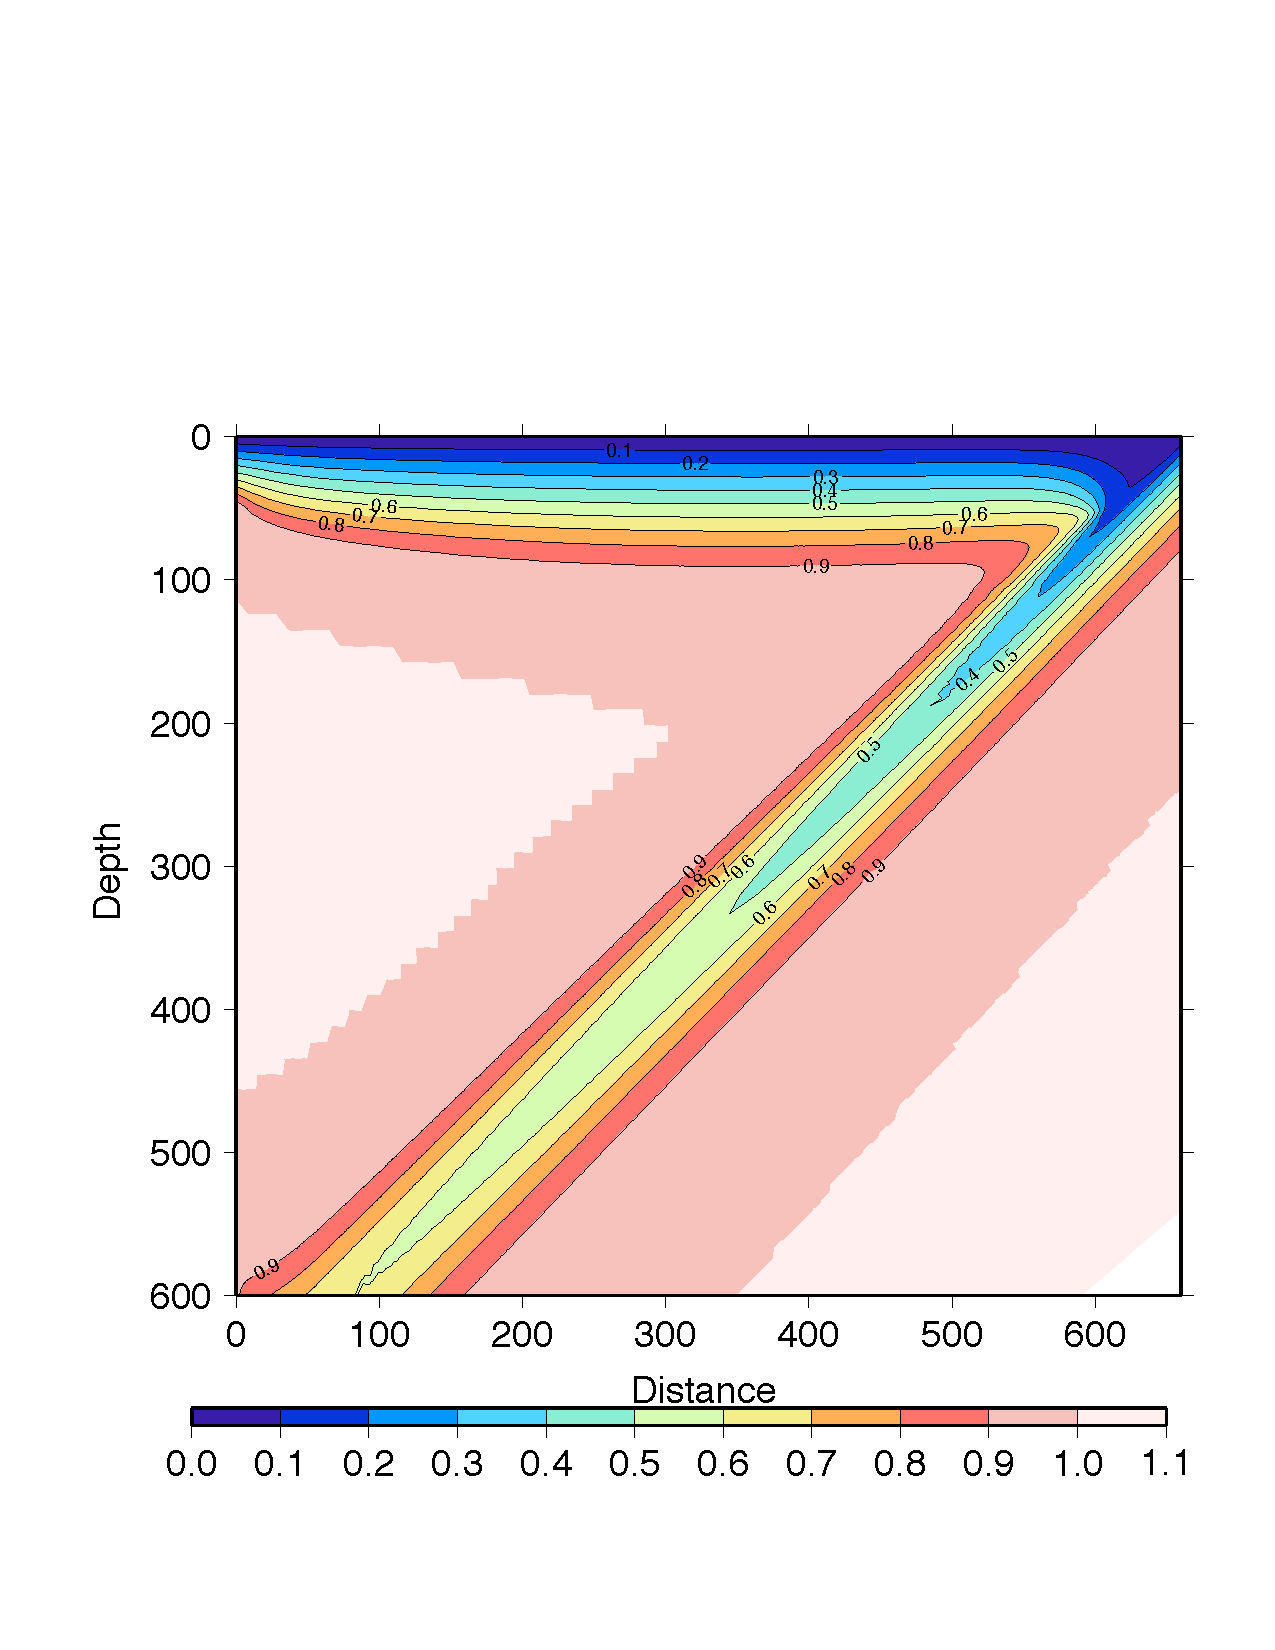
\includegraphics[scale=0.6]{images/wedge} 
\par\end{centering}
\end{figure}

\par\end{center}

\appendix
%dummy comment inserted by tex2lyx to ensure that this paragraph is not empty
%dummy comment inserted by tex2lyx to ensure that this paragraph is not empty
%dummy comment inserted by tex2lyx to ensure that this paragraph is not empty



\chapter{License }

\textbf{GNU GENERAL PUBLIC LICENSE Version 2, June 1991. Copyright
(C) 1989, 1991 Free Software Foundation, Inc. 59 Temple Place, Suite
330, Boston, MA 02111-1307 USA} \\
 Everyone is permitted to copy and distribute verbatim copies of this
license document, but changing it is not allowed.


\section*{Preamble}

The licenses for most software are designed to take away your freedom
to share and change it. By contrast, the GNU General Public License
is intended to guarantee your freedom to share and change free software
-- to make sure the software is free for all its users. This General
Public License applies to most of the Free Software Foundation's software
and to any other program whose authors commit to using it. (Some other
Free Software Foundation software is covered by the GNU Library General
Public License instead.) You can apply it to your programs, too.

When we speak of free software, we are referring to freedom, not price.
Our General Public Licenses are designed to make sure that you have
the freedom to distribute copies of free software (and charge for
this service if you wish), that you receive source code or can get
it if you want it, that you can change the software or use pieces
of it in new free programs; and that you know you can do these things.

To protect your rights, we need to make restrictions that forbid anyone
to deny you these rights or to ask you to surrender the rights. These
restrictions translate to certain responsibilities for you if you
distribute copies of the software, or if you modify it.

For example, if you distribute copies of such a program, whether gratis
or for a fee, you must give the recipients all the rights that you
have. You must make sure that they, too, receive or can get the source
code. And you must show them these terms so they know their rights.

We protect your rights with two steps:

\begin{enumerate}
\item Copyright the software, and 
\item Offer you this license which gives you legal permission to copy, distribute
and/or modify the software. 
\end{enumerate}
Also, for each author's protection and ours, we want to make certain
that everyone understands that there is no warranty for this free
software. If the software is modified by someone else and passed on,
we want its recipients to know that what they have is not the original,
so that any problems introduced by others will not reflect on the
original authors' reputations.

Finally, any free program is threatened constantly by software patents.
We wish to avoid the danger that redistributors of a free program
will individually obtain patent licenses, in effect making the program
proprietary. To prevent this, we have made it clear that any patent
must be licensed for everyone's free use or not licensed at all.

The precise terms and conditions for copying, distribution and modification
follow.


\section*{GNU GENERAL PUBLIC LICENSE TERMS AND CONDITIONS FOR COPYING, DISTRIBUTION
AND MODIFICATION }

\begin{itemize}
\item [0.]This License applies to any program or other work which contains
a notice placed by the copyright holder saying it may be distributed
under the terms of this General Public License. The \char`\"{}Program\char`\"{}
below refers to any such program or work, and a \char`\"{}work based
on the Program\char`\"{} means either the Program or any derivative
work under copyright law: that is to say, a work containing the Program
or a portion of it, either verbatim or with modifications and/or translated
into another language. (Hereinafter, translation is included without
limitation in the term \char`\"{}modification.\char`\"{}) Each licensee
is addressed as \char`\"{}you.\char`\"{}\\
 \\
 Activities other than copying, distribution and modification are
not covered by this License; they are outside its scope. The act of
running the Program is not restricted, and the output from the Program
is covered only if its contents constitute a work based on the Program
(independent of having been made by running the Program). Whether
that is true depends on what the Program does. 
\end{itemize}
\begin{enumerate}
\item You may copy and distribute verbatim copies of the Program's source
code as you receive it, in any medium, provided that you conspicuously
and appropriately publish on each copy an appropriate copyright notice
and disclaimer of warranty; keep intact all the notices that refer
to this License and to the absence of any warranty; and give any other
recipients of the Program a copy of this License along with the Program.


You may charge a fee for the physical act of transferring a copy,
and you may at your option offer warranty protection in exchange for
a fee.

\item You may modify your copy or copies of the Program or any portion of
it, thus forming a work based on the Program, and copy and distribute
such modifications or work under the terms of Section 1 above, provided
that you also meet all of these conditions:

\begin{enumerate}
\item You must cause the modified files to carry prominent notices stating
that you changed the files and the date of any change. 
\item You must cause any work that you distribute or publish, that in whole
or in part contains or is derived from the Program or any part thereof,
to be licensed as a whole at no charge to all third parties under
the terms of this License. 
\item If the modified program normally reads commands interactively when
run, you must cause it, when started running for such interactive
use in the most ordinary way, to print or display an announcement
including an appropriate copyright notice and a notice that there
is no warranty (or else, saying that you provide a warranty) and that
users may redistribute the program under these conditions, and telling
the user how to view a copy of this License. (Exception: if the Program
itself is interactive but does not normally print such an announcement,
your work based on the Program is not required to print an announcement.) 
\end{enumerate}
These requirements apply to the modified work as a whole. If identifiable
sections of that work are not derived from the Program, and can be
reasonably considered independent and separate works in themselves,
then this License, and its terms, do not apply to those sections when
you distribute them as separate works. But when you distribute the
same sections as part of a whole which is a work based on the Program,
the distribution of the whole must be on the terms of this License,
whose permissions for other licensees extend to the entire whole,
and thus to each and every part regardless of who wrote it.

Thus, it is not the intent of this section to claim rights or contest
your rights to work written entirely by you; rather, the intent is
to exercise the right to control the distribution of derivative or
collective works based on the Program.

In addition, mere aggregation of another work not based on the Program
with the Program (or with a work based on the Program) on a volume
of a storage or distribution medium does not bring the other work
under the scope of this License.

\item You may copy and distribute the Program (or a work based on it, under
Section 2) in object code or executable form under the terms of Sections
1 and 2 above provided that you also do one of the following:

\begin{enumerate}
\item Accompany it with the complete corresponding machine-readable source
code, which must be distributed under the terms of Sections 1 and
2 above on a medium customarily used for software interchange; or, 
\item Accompany it with a written offer, valid for at least three years,
to give any third party, for a charge no more than your cost of physically
performing source distribution, a complete machine-readable copy of
the corresponding source code, to be distributed under the terms of
Sections 1 and 2 above on a medium customarily used for software interchange;
or, 
\item Accompany it with the information you received as to the offer to
distribute corresponding source code. (This alternative is allowed
only for noncommercial distribution and only if you received the program
in object code or executable form with such an offer, in accord with
Subsection b above.) 
\end{enumerate}
The source code for a work means the preferred form of the work for
making modifications to it. For an executable work, complete source
code means all the source code for all modules it contains, plus any
associated interface definition files, plus the scripts used to control
compilation and installation of the executable. However, as a special
exception, the source code distributed need not include anything that
is normally distributed (in either source or binary form) with the
major components (compiler, kernel, and so on) of the operating system
on which the executable runs, unless that component itself accompanies
the executable.

If distribution of executable or object code is made by offering access
to copy from a designated place, then offering equivalent access to
copy the source code from the same place counts as distribution of
the source code, even though third parties are not compelled to copy
the source along with the object code.

\item You may not copy, modify, sublicense, or distribute the Program except
as expressly provided under this License. Any attempt otherwise to
copy, modify, sublicense or distribute the Program is void, and will
automatically terminate your rights under this License. However, parties
who have received copies, or rights, from you under this License will
not have their licenses terminated so long as such parties remain
in full compliance. 
\item You are not required to accept this License, since you have not signed
it. However, nothing else grants you permission to modify or distribute
the Program or its derivative works. These actions are prohibited
by law if you do not accept this License. Therefore, by modifying
or distributing the Program (or any work based on the Program), you
indicate your acceptance of this License to do so, and all its terms
and conditions for copying, distributing or modifying the Program
or works based on it. 
\item Each time you redistribute the Program (or any work based on the Program),
the recipient automatically receives a license from the original licensor
to copy, distribute or modify the Program subject to these terms and
conditions. You may not impose any further restrictions on the recipients'
exercise of the rights granted herein. You are not responsible for
enforcing compliance by third parties to this License. 
\item If, as a consequence of a court judgment or allegation of patent infringement
or for any other reason (not limited to patent issues), conditions
are imposed on you (whether by court order, agreement or otherwise)
that contradict the conditions of this License, they do not excuse
you from the conditions of this License. If you cannot distribute
so as to satisfy simultaneously your obligations under this License
and any other pertinent obligations, then as a consequence you may
not distribute the Program at all. For example, if a patent license
would not permit royalty-free redistribution of the Program by all
those who receive copies directly or indirectly through you, then
the only way you could satisfy both it and this License would be to
refrain entirely from distribution of the Program.


If any portion of this section is held invalid or unenforceable under
any particular circumstance, the balance of the section is intended
to apply and the section as a whole is intended to apply in other
circumstances.

It is not the purpose of this section to induce you to infringe any
patents or other property right claims or to contest validity of any
such claims; this section has the sole purpose of protecting the integrity
of the free software distribution system, which is implemented by
public license practices. Many people have made generous contributions
to the wide range of software distributed through that system in reliance
on consistent application of that system; it is up to the author/donor
to decide if he or she is willing to distribute software through any
other system and a licensee cannot impose that choice.

This section is intended to make thoroughly clear what is believed
to be a consequence of the rest of this License.

\item If the distribution and/or use of the Program is restricted in certain
countries either by patents or by copyrighted interfaces, the original
copyright holder who places the Program under this License may add
an explicit geographical distribution limitation excluding those countries,
so that distribution is permitted only in or among countries not thus
excluded. In such case, this License incorporates the limitation as
if written in the body of this License. 
\item The Free Software Foundation may publish revised and/or new versions
of the General Public License from time to time. Such new versions
will be similar in spirit to the present version, but may differ in
detail to address new problems or concerns.


Each version is given a distinguishing version number. If the Program
specifies a version number of this License which applies to it and
\char`\"{}any later version,\char`\"{} you have the option of following
the terms and conditions either of that version or of any later version
published by the Free Software Foundation. If the Program does not
specify a version number of this License, you may choose any version
ever published by the Free Software Foundation.

\item If you wish to incorporate parts of the Program into other free programs
whose distribution conditions are different, write to the author to
ask for permission. For software which is copyrighted by the Free
Software Foundation, write to the Free Software Foundation; we sometimes
make exceptions for this. Our decision will be guided by the two goals
of preserving the free status of all derivatives of our free software
and of promoting the sharing and reuse of software generally. 
\end{enumerate}

\subsection*{NO WARRANTY }

\begin{itemize}
\item [11.]BECAUSE THE PROGRAM IS LICENSED FREE OF CHARGE, THERE IS NO
WARRANTY FOR THE PROGRAM, TO THE EXTENT PERMITTED BY APPLICABLE LAW.
EXCEPT WHEN OTHERWISE STATED IN WRITING THE COPYRIGHT HOLDERS AND/OR
OTHER PARTIES PROVIDE THE PROGRAM \char`\"{}AS IS\char`\"{} WITHOUT
WARRANTY OF ANY KIND, EITHER EXPRESSED OR IMPLIED, INCLUDING, BUT
NOT LIMITED TO, THE IMPLIED WARRANTIES OF MERCHANTABILITY AND FITNESS
FOR A PARTICULAR PURPOSE. THE ENTIRE RISK AS TO THE QUALITY AND PERFORMANCE
OF THE PROGRAM IS WITH YOU. SHOULD THE PROGRAM PROVE DEFECTIVE, YOU
ASSUME THE COST OF ALL NECESSARY SERVICING, REPAIR OR CORRECTION. 
\item [12.]IN NO EVENT UNLESS REQUIRED BY APPLICABLE LAW OR AGREED TO
IN WRITING WILL ANY COPYRIGHT HOLDER, OR ANY OTHER PARTY WHO MAY MODIFY
AND/OR REDISTRIBUTE THE PROGRAM AS PERMITTED ABOVE, BE LIABLE TO YOU
FOR DAMAGES, INCLUDING ANY GENERAL, SPECIAL, INCIDENTAL OR CONSEQUENTIAL
DAMAGES ARISING OUT OF THE USE OR INABILITY TO USE THE PROGRAM (INCLUDING
BUT NOT LIMITED TO LOSS OF DATA OR DATA BEING RENDERED INACCURATE
OR LOSSES SUSTAINED BY YOU OR THIRD PARTIES OR A FAILURE OF THE PROGRAM
TO OPERATE WITH ANY OTHER PROGRAMS), EVEN IF SUCH HOLDER OR OTHER
PARTY HAS BEEN ADVISED OF THE POSSIBILITY OF SUCH DAMAGES. 
\end{itemize}

\section*{END OF TERMS AND CONDITIONS }


\subsection*{How to Apply These Terms to Your New Programs}

If you develop a new program, and you want it to be of the greatest
possible use to the public, the best way to achieve this is to make
it free software which everyone can redistribute and change under
these terms.

To do so, attach the following notices to the program. It is safest
to attach them to the start of each source file to most effectively
convey the exclusion of warranty; and each file should have at least
the \char`\"{}copyright\char`\"{} line and a pointer to where the
full notice is found. For example:

\begin{quote}
One line to give the program's name and a brief idea of what it does.
Copyright {\footnotesize � (}year) (name of author)

This program is free software; you can redistribute it and/or modify
it under the terms of the GNU General Public License as published
by the Free Software Foundation; either version 2 of the License,
or (at your option) any later version.

This program is distributed in the hope that it will be useful, but
WITHOUT ANY WARRANTY; without even the implied warranty of MERCHANTABILITY
or FITNESS FOR A PARTICULAR PURPOSE. See the GNU General Public License
for more details.

You should have received a copy of the GNU General Public License
along with this program; if not, write to the Free Software Foundation,
Inc., 59 Temple Place, Suite 330, Boston, MA 02111-1307 USA 
\end{quote}
Also add information on how to contact you by electronic and paper
mail.

If the program is interactive, make it output a short notice like
this when it starts in an interactive mode:

\begin{quote}
Gnomovision version 69, Copyright � year name of author Gnomovision
comes with ABSOLUTELY NO WARRANTY; for details type `show w'. This
is free software, and you are welcome to redistribute it under certain
conditions; type `show c' for details. 
\end{quote}
The hypothetical commands `show w' and `show c' should show the appropriate
parts of the General Public License. Of course, the commands you use
may be called something other than `show w' and `show c'; they could
even be mouse-clicks or menu items -- whatever suits your program.

You should also get your employer (if you work as a programmer) or
your school, if any, to sign a \char`\"{}copyright disclaimer\char`\"{}
for the program, if necessary. Here is a sample; alter the names:

\begin{quote}
Yoyodyne, Inc., hereby disclaims all copyright interest in the program
`Gnomovision' (which makes passes at compilers) written by James Hacker.

(signature of Ty Coon)\\
 1 April 1989 \\
 Ty Coon, President of Vice 
\end{quote}
This General Public License does not permit incorporating your program
into proprietary programs. If your program is a subroutine library,
you may consider it more useful to permit linking proprietary applications
with the library. If this is what you want to do, use the GNU Library
General Public License instead of this License.

\begin{thebibliography}{10}
\bibitem[1]{Blankenbach et al, 1989}Blankenbach, B., F. Busse, U.
Christensen, L. Cserepes, D. Gunkel, U. Hansen, H. Harder, G. Jarvis,
M. Koch, G. Marquart, D. Moore, P. Olson, H. Schmeling and T. Schnaubelt
(1989) A Benchmark comparison for mantle convection codes, \emph{Geophys.
J. Int.}, 98, 23-38.

\bibitem[2]{Brooks 1981}Brooks, A.N. \emph{A Petrov-Galerkin finite-element
formulation for convection dominated flows.} Unpublished doctoral
thesis, California Institute of Technology, Pasadena, CA, 1981.

\bibitem[3]{Brooks and Hughes 1990}Brooks, A.N. and Hughes, T.J.R.
(1990), Streamline upwind/Petrov-Galerkin formulations for convection
dominated flows with particular emphasis on the incompressible Navier-Stokes
equations. \emph{Comp. Meth. in Appl. Mech. and Eng., 81(3),} 199-259.

\bibitem[4]{Hughes 1987}Hughes, T.J.R. \emph{The finite element method.}
Prentice-Hall, Inc., Englewood Cliffs, New Jersey, 1987.

\bibitem[5]{Hughes and Brooks 1979}Hughes, T.J.R. and Brooks, A.N.
(1979), A multi-dimensional upwind scheme with no crosswind diffusion.
In: Finite element methods for convection dominated flows (T.J.R.
Hughes, ed.), \emph{ASME,} \emph{34}, 19-35.

\bibitem[6]{Hughes et al 1988}Hughes, T.J.R., Franca, L.P., Hulbert,
G.M., Johan, Z., and Shakib, F. (1988), The Galerkin/least-squares
method for advective-diffusive equations, in \emph{Recent developments
in computational fluid dynamics} (T.E. Tezduyar, ed.), \emph{ASME,}
\emph{95}, 75-99.

\bibitem[7]{Hughes et al 1979}Hughes, T.J.R., Liu, W.K., and Brooks,
A.N. (1979), Finite element analysis of incompressible viscous flows
by the penalty function formulation. \emph{J. Comput. Phys.,} \emph{30},
1-60.

\bibitem[8]{Malkus and Hughes 1978}Malkus, D.S. and Hughes, T.J.R.
(1978), Mixed finite element methods reduced and selective integration
techniques: a unification of concepts. \emph{Comp. Meth. in Appl.
Mech. and Eng.,} \emph{15}, 63-81.

\bibitem[9]{Temam 1977}Temam, R. \emph{Navier-Stokes equations: theory
and numerical analysis}. North-Holland. Amsterdam, 1977.

\bibitem[10]{Travis et al 1990}Travis, B.J., Anderson, C., Baumgardner,
J., Gable, C.W., Hager, B.H., O'Connell, R.J., Olson, P., Raefsky,
A. and Schubert, G. (1990), A benchmark comparison of numerical methods
for infinite Prandtl number convection in two-dimensional Cartesian
geometry, \emph{Geophys. Astrophys. Fluid Dynamics,} \emph{55}, 137-160,
doi: 10.1080/03091929008204111

\bibitem[11]{van Keken 1993}van Keken, P. E. (1993) Numerical modeling
of thermochemically driven fluid flow with non-Newtonian rheology:
Applied to the Earth's lithosphere and mantle, Ph.D. Thesis, Utrecht
University.

\bibitem[12]{van Keken et al 2008} van Keken, P.E., Currie, C., King,
S.D., Behn, M.D., Canioncle, A., He, J., Katz, R.F., Lin, S.-C., Parmentier,
E.M., Spiegelman, M., and Wang, K. (2008), A community benchmark for
subduction zone modeling, \emph{Phys. Earth Planet. Int.}, in press. 
\end{thebibliography}

\end{document}
